\documentclass[landscape]{beamer}
\usepackage[bookmarks=true]{hyperref}
\usepackage{algorithm}
\usepackage{graphics}
\usepackage[noEnd=false,indLines=false]{algpseudocodex}
\usetheme{Copenhagen}
%\usetheme{metropolis}
\usepackage{bookmark}
\usepackage{amsmath}
\usepackage{amsfonts}
\usepackage{bm}
\usepackage{colortbl}
\usepackage{subcaption}
\captionsetup[subfigure]{labelformat=simple}
\renewcommand{\thesubfigure}{(\alph{subfigure})}
\usepackage{multirow}
\usepackage{url}
\usepackage{placeins}
\usepackage{hhline}
\usepackage{colonequals}
\usepackage{tikz}
\usepackage{kbordermatrix}
% \usepackage[pagewise]{lineno}
% \linenumbers
% \usepackage{draftwatermark}
% \SetWatermarkText{DRAFT}
% \SetWatermarkScale{1}
\DeclareMathOperator*{\argmin}{arg\,min}
\renewcommand{\topfraction}{1}
\renewcommand{\bottomfraction}{1}
\renewcommand{\textfraction}{0}
\newcommand{\R}{{\mathbb R}}
\newcommand{\C}{{\mathbb C}}
\newcommand{\N}{{\mathbb N}}
\newcommand{\Z}{{\mathbb Z}}
% \newcommand{\alt}{\mathrel{
%     \raisebox{-.75ex}{$\mathop{\sim}\limits^{\textstyle <}$}}}
\newcommand{\dia}{{\rm diag}}
\newcommand{\trace}{\operatorname{tr}}
\newcommand{\adj}{^{*}}
\newcommand{\inv}{^{-1}}
\newcommand{\itp}{^{\rm -T}}
\newcommand{\unv}{{\bf e}}
\newcommand{\exc}{{\rm exc}}
\newcommand{\real}{\mbox{\rm Re}}
\newcommand{\dist}{\mbox{\rm dist}}
\newcommand{\imag}{\mbox{\rm Imag}}
\newcommand{\conj}[1]{\overline{#1}}
\newcommand{\fl}{\mbox{fl}}
\newcommand{\op}{\, \mbox{op}\,}
\newcommand{\sign}{\mbox{sign}}
\newcommand{\vspan}{R}
\newcommand{\eqand}{\qquad\mbox{and}\qquad}
\newcommand{\rank}{{\rm rank}}
\newcommand{\range}{\mathcal{R}}
\newcommand{\nullspace}{\mbox{null}}
\newcommand{\lnull}{\mbox{lnull}}
\newcommand{\rnull}{\mbox{null}}
\renewcommand{\vec}[1]{\bm{#1}}
\newcommand{\ts}{\textsuperscript}
\newcommand{\T}{{\rm T}}
\newcommand{\pT}{{\prime\, \T}}
\renewcommand{\H}{{\rm H}}
\newcommand{\e}[1]{\mbox{e}{#1}}
%\newcommand{\e}[1]{\times 10^{#1}}
\newcommand{\mstrut}{\rule{0pt}{1.2em}}
\newenvironment{mtx}[1]{\left[\begin{array}{#1}}{\end{array}\right]}
\newcommand{\mcal}[1]{\mathcal{#1}}
\DeclareMathOperator{\Gr}{Gr}
\DeclareMathOperator{\grad}{grad}
\DeclareMathOperator{\hess}{Hess}

\setbeamertemplate{navigation symbols}{}
% Put paragraph indentation in enumerate environment.
\let\oldenumerate=\enumerate
\renewenvironment{enumerate}{\oldenumerate\parindent=1.5em}{\endlist}
\usepackage[displaymath,textmath,sections,graphics]{preview}
\PreviewEnvironment{align*}
\PreviewEnvironment{multline*}
\PreviewEnvironment{tabular}
\PreviewEnvironment{verbatim}
\PreviewEnvironment{lstlisting}
\PreviewEnvironment*{frame}
\PreviewEnvironment*{algorithmic}
% \PreviewEnvironment*{minipage}

\usefonttheme[onlymath]{serif}

\title[Spectral Transformation Lanczos Algorithm]{Spectral Transformation Lanczos Algorithm for the
  Symmetric Definite Generalized Eigenvalue Problem}
  \author{Ayobami Adebesin}
\date{April 8th, 2025}

\begin{document}

\begin{frame}
  \titlepage

\end{frame}

\begin{frame}
  \frametitle{Problem Statement}

  \begin{block}{The Symmetric Definite Generalized Eigenvalue Problem}
    For $n\times n$ real matrices $A=A^\T$ and positive definite (or
    semidefinite) $B=B^\T$, find $\vec{v}\neq \vec{0}$ and $\lambda$
    such that
    \begin{equation*}
      A\vec{v} = \lambda B\vec{v}
    \end{equation*}
    where $\mcal{N}(A)\cap \mcal{N}(B)=\{\vec{0}\}$.  The value
    $\lambda$ is a generalized eigenvalue and $\vec{v}$ is the
    corresponding generalized eigenvector.  If $B$ is invertible, the
    generalized eigenvalues are eigenvalues for
    $B^{-1}A\vec{v} = \lambda \vec{v}$.  Otherwise, for
    $B\vec{v}=\vec{0}$, we say that $\lambda = \infty$ is an
    eigenvalue.  If $B$ is positive definite, there are $n$ linearly
    independent eigenvectors.
  \end{block}
  
  We assume throughout that $A\neq 0$ and $B\neq 0$.
\end{frame}

\begin{frame}
  \frametitle{Applications and Algorithms}

  \begin{itemize}
  \item Vibration Analysis in Structural engineering e.g (Boeing).
  
  For example, equation of a vibrating system:
  \begin{equation*}
  	K\mathbf{x} = \lambda M\mathbf{x}
  \end{equation*}
  where $M$ is the mass matrix, $K$ is the stiffness matrix, $\mathbf{x}$ is the displacement vector, and $\lambda$ is the eigenfrequencies of the system.
  \item Existing factorization algorithms for the dense problem all
    have performance and/or stability issues.
  \item Recent work on direct methods have proven residual bounds for dense problems. [Michael Stewart, 2024].
  \item This work is about applying an iterative method to the sparse problem, and verifying the residual bounds predicted by direct methods.
  \item We start with a survey of existing methods.
  \end{itemize}
\end{frame}

\begin{frame}
  \frametitle{The Standard Algorithm\\
    (J.H. Wilkinson, 1965)}
  
  If $B$ is positive definite then it has a Cholesky factor
  \begin{equation*}
    B = C_b C_b^\T.
  \end{equation*}
  Thus
  \begin{equation*}
    \begin{array}{l}
      A \vec{v} = \lambda B\vec{v} \\
      \Leftrightarrow A \vec{v} = \lambda C_b C_b^\T \vec{v} \\
      \Leftrightarrow C_b^{-1} A C_b^{-\T} C_b^\T \vec{v} = \lambda C_b^{\T} \vec{v}.
    \end{array}
  \end{equation*}

  \begin{block}{Standard Reduction to an Ordinary Eigenvalue Problem}
    Solve the symmetric eigenvalue problem
    \begin{equation*}
      C_b^{-1} A C_b^{-\T} \vec{u} = \lambda \vec{u}, \qquad \vec{u} \neq \vec{0}
    \end{equation*}
    Then solve $C_b^\T\vec{v} = \vec{u}$.
  \end{block}
\end{frame}

\begin{frame}
  \frametitle{The Standard Algorithm (cont'd)}

  \begin{itemize}
  \item This shows that the symmetric definite generalized eigenvalue
    problem has real eigenvalues.  Eigenvectors are orthogonal with
    respect to the inner product
    $(\vec{x}, \vec{y}) = \vec{y}^\T B \vec{x}$.
  \item It is fast and it is the approach used by LAPACK.
  \item It fails if $B$ is semidefinite and is unstable when $B$ is
    ill-conditioned (i.e. $\kappa_2(B) = \|B\|_2\|B^{-1}\|_2$ is
    large.)
  \item If $B$ is ill-conditioned, it usually delivers small residuals for large eigenvalues and large residuals for small eigenvalues. 
  \item There are alternatives, each with its own set of problems\ldots
  \end{itemize}
\end{frame}

\begin{frame}
  \frametitle{An Alternate Formulation}
  The generalized eigenvalue problem can be formulated in another way as follows:

  \begin{block}{The Generalized Eigenvalue Problem Version II}
    The eigenvalue problem can be written
    \begin{equation*}
      \beta A \vec{v} = \alpha B \vec{v}
    \end{equation*}
    where $\vec{v} \neq \vec{0}$ and $\beta$ and $\alpha$ are not both
    zero.  The original formulation eigenvalues are given by
    $\lambda = \alpha/\beta$.  Each eigenvalue is a nonunique pair
    $(\alpha, \beta)$ that can be scaled by $c \neq 0$.  It
    can be identified with a subspace of $\R^2$ (or $\C^2$):
    \begin{equation*}
      \mathcal{E} = 
      \left\{ c\cdot (\alpha, \beta) : c \in \R \right\}
    \end{equation*}
  \end{block}
\end{frame}


\begin{frame}
\frametitle{The $QZ$ Algorithm I \\
  (C. B. Moler and G. W. Stewart, 1972)}

\begin{block}{Generalized Schur Form}
  For $A$ and $B$ not necessarily symmetric, there exist unitary $Q$
  and $Z$ such that
  \begin{equation*}
    Q^H A Z = T_a, \qquad
    Q^H B Z = T_b.
  \end{equation*}
  where $T_a$ and $T_b$ are upper triangular with diagonal elements
  $\alpha_i$ and $\beta_i$.  The eigenvalues for
  $A\vec{v} = \lambda B\vec{v}$ are given by
  $\lambda_i = \alpha_{i}/\beta_{i}$.  Eigenvectors can be obtained from $Z$
  with additional computation.
\end{block}

\begin{itemize}
\item With rounding, the $QZ$ algorithm for computing this is backward
  stable: There exist exactly unitary $\tilde{Q}$ and $\tilde{Z}$
  close to the computed $Q$ and $Z$ for which the computed $T_a$ and
  $T_b$ satisfy
  \begin{equation*}
    \tilde{Q}^H (A+E) \tilde{Z} = T_a , \qquad
    \tilde{Q}^H (B+F) \tilde{Z} = T_b.
  \end{equation*}
\end{itemize}
\end{frame}

\begin{frame}
  \frametitle{More on the $QZ$ Algorithm}

  \begin{itemize}
  \item The errors satisfy $\|E\| = O(u)\|A\|$ and
    $\|F\| = O(u)\|B\|$, where $u$ is the unit roundoff.
    ($u\approx 10^{-16}$ for double precision.)
  \item The pairs $(\alpha_{i},\beta_{i})$ are exact generalized
    eigenvalues of matrices close to $A$ and $B$.
  \item The algorithm is much slower than the standard algorithm.
  \item Unfortunately $E$ and $F$ are not guaranteed to be symmetric
    even when $A$ and $B$ are.  The computed eigenvalues can even have
    imaginary parts that are not small.  Simply truncating the imaginary
    part does not give satisfactory results.
  \end{itemize}
\end{frame}

\begin{frame}
  \frametitle{Diagonalization Using Congruences \\
  S. Chandrasekaran 2000}

\begin{block}{Diagonalization}
  For the symmetric definite problem there exists nonsingular $Z$ such that
  \begin{equation*}
    A = Z D_a Z^\T, \qquad B = Z D_b Z^\T.
  \end{equation*}
  If $\alpha_i$ and $\beta_i$ are the diagonal elements of $D_a$ and
  $D_b$, then the generalized eigenvalues are $(\alpha_i, \beta_i)$ or
  $\lambda_i = \alpha_i/ \beta_i$.  The eigenvectors are the columns
  of $V= Z^{-\T}$.
\end{block}

\begin{itemize}
\item It can be shown that $V=Z^{-\T}$ is a good eigenvector matrix.
\item It is as close to ideal numerically as any current algorithm.
\item It involves solving multiple ordinary eigenvalue problems and its
  complexity is not proven to be $O(n^3)$.
\end{itemize}
\end{frame}

\begin{frame}
  \frametitle{Spectral Transformation Lanczos
    [T. Ericsson and A. Ruhe, 1980]}

  \begin{lemma}
    \label{lm:spectral_transformation}
    Let $\lambda = \alpha/\beta \neq \infty$ and $\vec{v}\neq 0$ satisfy
    $A\vec{v} = \lambda B \vec{v}$.  Assume that $A-\sigma B$ is nonsingular and
    $B = C_b C_b^\T$, $C_b \in \mathbb{R}^{n \times r}$ with linearly independent
    columns.  Then $\theta = 1/(\lambda-\sigma)$ is an eigenvalue of
    the shifted and inverted problem
    \begin{equation*}
      C_b^\T (A-\sigma B)^{-1} C_b \vec{u} = \theta \vec{u}, \qquad \vec{u}\neq \vec{0}.
    \end{equation*}
    with eigenvector $\vec{u} = C_b^\T \vec{v}\neq \vec{0}$.

    Conversely, assume that $\vec{u}\neq \vec{0}$ is an eigenvector
    for the shifted and inverted problem with eigenvalue $\theta$.
    Then the vector $\vec{v} = (A - \sigma B)^{-1} C_b \vec{u}\neq 0$
    is an eigenvector for the eigenvalue $(1 + \sigma \theta, \theta)$
    of the original problem.
  \end{lemma}
\end{frame}

\begin{frame}
	\frametitle{Spectral Transformation for Dense Problems [Michael Stewart, 2024]}
	This direct method employs the spectral transformation described by [T. Ericsson and A. Ruhe, 1980], and symmetric decompositions of $A- \sigma B$ and $B$ such that
	\begin{equation*}
		A-\sigma B = C_a D C_a^\T, \eqand B = C_b C_b^\T,
	\end{equation*} 
	to transform the problem into a symmetric standard eigenvalue problem given by
	\begin{equation*}
		C_b^\T C_a^{-T} D_a C_a^{-1} C_b \vec{u} = \theta \vec{u},\qquad 
		\vec{v} = C_a^{-\T} D_a C_a^{-1} C_b \vec{u}
	\end{equation*}
	with $(\alpha, \beta) = (1+\sigma \theta, \theta)$ or $\lambda = (1+\sigma\theta)/\theta$.
	
	\begin{itemize}
		\item $B$ can factored using pivoted Cholesky and $A$ using $LDL^\T$
		factorization with rook pivoting, both available in LAPACK.
		\item We cannot expect a shift to result in well conditioned
		$A-\sigma B$ or $C_a$,  {\bf but ill conditioning is not what matters!}
	\end{itemize}
\end{frame}

\begin{frame}
	\frametitle {Interesting Questions}
	\begin{center}
		\begin{itemize}
			\item \large Do the residual bounds proven for a direct method applies when an iterative method is used for the spectral transformed problem?
			\item \large Does the spectral transformed problem respects symmetry in the decomposition of $A - \sigma B$?
		\end{itemize}
	\end{center}
\end{frame}

\begin{frame}
	\frametitle{What is our approach?}
	\begin{itemize}
		\item Apply the Lanczos algorithm to the spectral problem
		\item Investigate if the residuals for the computed eigenvalues follows the bounds for the direct methods in terms of the choice of shift?
		\item Explore the effect of symmetric decomposition of $A- \sigma B$ on residuals
	\end{itemize}
\end{frame}

\begin{frame}[allowframebreaks]{Outline}
	\frametitle{Spectral Transformation Lanczos Algorithm}
	
	\begin{algorithmic}[1]
		\Function{\textsc{Spectral\_Lanczos}}{$A, B, m, n, \sigma, tol$}
		\State Choose an arbitrary vector $\mathbf{b}$ and set an initial vector $\mathbf{q_1} = \mathbf{b}/ \|\mathbf{b}\|_2$
		\State Set $\beta_0 = 0$ and $\mathbf{q_0} = \mathbf{0}$
		\State Set $Q = \text{zeros}(m, n+1)$
		\State Precompute the $LU$ factorization of $A - \sigma B$: $LU = (A - \sigma B)$
		\State Factor: $B = CC^T$
		\For{$j = 1, 2, \dots, n$}
		\State $Q[:, j] = \mathbf{q}_j$
		\State $\mathbf{u} = C\mathbf{q}_j$
		\State Solve: $(LU)\mathbf{v} = \mathbf{u}$ for $\mathbf{v}$
		\pause
		\State $\mathbf{v} = C^T \mathbf{v}$
		\If{$j < n $}
		\State $\alpha_j = \mathbf{q}_j^T \mathbf{v} $
		\State $\mathbf{v} = \mathbf{v} - \beta_{j-1}\mathbf{q}_{j-1} - \alpha_j \mathbf{q}_j$
		\State \textbf{Full reorthogonalization:} $\mathbf{v} = \mathbf{v} - \sum_{i \leq j} (\mathbf{q}_i^T \mathbf{v}) \mathbf{q}_i$
		\State $\beta_{j} = \|\mathbf{v}\|_2$
		\If{$\beta_{j} < tol $}
		\State \textbf{restart} or \textbf{exit}
		\EndIf
		\State $\mathbf{q}_{j+1} := \mathbf{v} / \beta_{j}$
		\EndIf
		\EndFor
		\State $Q = Q[:, :n]$
		\State $\mathbf{q} = Q[:, n]$
		\State \Return $(Q, T, \mathbf{q})$
		\EndFunction
	\end{algorithmic}
\end{frame}

\begin{frame}
  \frametitle{Some Definitions from [Michael Stewart, 2024]}

  \begin{equation*}
    X = C_a^{-1} C_b,  \qquad W = X^\T D_a X, \qquad
    \mu = \frac{\|X\|_2^2}{\|W\|_2} \geq 1.
  \end{equation*}
  \begin{equation*}
    \eta = \frac{\|A-\sigma B\|_2^{1/2}}{\|B\|_2^{1/2}},\qquad \sigma_0 = \sigma \frac{\|B\|_2}{\|A\|_2},
    \eqand \gamma = \frac{\|A\|_2}{\|A-\sigma B\|_2}.
  \end{equation*}
  
  \begin{itemize}
  \item The shifted and inverted problem is $W \vec{u} = \theta \vec{u}$.
  \item The only ``inversion'' is in solving $C_a X = C_b$.
  \item The values of $\mu$, $\eta \|X\|_2$, $\sigma_0$, and $\gamma$
    can potentially impact stability.
  \item $\eta \|X\|_2$ is the most interesting and important of these.
  \end{itemize}
\end{frame}

\begin{frame}
  \frametitle{Bounds for $\eta \|X\|_2$}

  We have
  \begin{equation*}
     \eta^2 \|X\|_2^2 \leq \mu \kappa_2(A-\sigma B)
  \end{equation*}
  and even better
  \begin{lemma}
    Assume that $\sigma \neq 0$ and $A-\sigma B$ is invertible.  Then
    \begin{align*}
      \eta^2 \|X\|_2^2 
      & \leq
      \left(1 + \frac{1}{|\sigma_0|}\right)
      \frac{\mu}{\min_i \left| 1 - \frac{\lambda_i}{\sigma}\right|} \\
      & = 
        (1 + |\sigma_0|)
        \frac{\mu}
        {\min_i \left|\frac{\|B\|_2}{\|A\|_2}\lambda_i - \sigma_0\right|}.
    \end{align*}
  \end{lemma}
\end{frame}

\begin{frame}
  \frametitle{Forward Errors}


  \begin{itemize}
  \item {\bf The size of $\eta^2 \|X\|_2^2$ determines stability and
      it is usually much smaller than $\kappa_2(A-\sigma B)$.}
  \item It is surprisingly easy to avoid large $\eta \|X\|_2$.  In
    practice, if $|\sigma_0|$ is not small, $\eta \|X\|_2$ is large
    only if $\sigma$ is chosen to match an eigenvalue $\lambda$ to
    several digits.  A random shift in a reasonable interval almost
    always works.
  \item If $A$ and $B$ are both positive definite, all generalized eigenvalues
    are positive, $\mu = 1$, and simply choosing $\sigma_0 = -1$ gives
    \begin{equation*}
      \eta^2 \|X\|_2^2 \leq 
      \left(1 + \frac{1}{1}\right) \frac{1}{\min_i \left| 1 + \frac{|\lambda_i|}{|\sigma|}\right|} \leq 2
    \end{equation*}

  \end{itemize}
\end{frame}


\begin{frame}
  \frametitle{Error Bounds: Moderate Shifts and Eigenvalue Stability}

  \begin{block}{Eigenvalue Backward Errors}
    For the computed $\theta_i$, there exist symmetric $E$ and $F$ and
    a vector $\tilde{\vec{v}}_i\neq \vec{0}$ such that
    \begin{equation*}
      \theta_i (A+E) \tilde{\vec{v}}_i = (1+\sigma \theta_i) (B+F) \tilde{\vec{v}}_i
    \end{equation*}
    and
    \begin{equation*}
      \max\left(\frac{\|E\|_2}{\|A\|_2}, \frac{\|F\|_2}{\|B\|_2}\right) \leq 
      O(u) (1+|\sigma_0|) \eta^2 \|X\|_2^2 + O(u^2)
    \end{equation*}
  \end{block}

  If $|\sigma_0|$ is not large and $\eta^2 \|X\|_2^2$ is not large, each
  $(1+\sigma \theta_i, \theta_i)$ is an eigenvalue of a pair close to $(A,B)$.
\end{frame}

\begin{frame}
  \frametitle{Error Bounds: Moderate Shifts with Computed Eigenvectors}

  \begin{block}{Computed Eigenvector Bounds}
    There exist symmetric
    $E$ and $F$ such that the computed $\theta_i$ and the computed
    eigenvector $\vec{v}_i$ satisfy
    \begin{equation*}
      \theta_i (A+E) \vec{v}_i = (1+\sigma \theta_i) (B+F) \vec{v}_i
    \end{equation*}
    with
    \begin{multline*}
      \max\left(\frac{\|E\|_2}{\|A\|_2}, \frac{\|F\|_2}{\|B\|_2}\right) \leq \\
      O(u) |1-\lambda_i/\sigma| |\sigma_0| \left(1 + \max(\gamma,1)
      \left(1+ |1-\lambda_i/\sigma|\right)\eta^2\|X\|_2^2\right) +O(u^2)
    \end{multline*}
  \end{block}
  
  If $|\sigma_0|$ and $\eta^2 \|X\|_2^2$ are not large, $A-\sigma B$
  does not cancel, and $\lambda_i = (1+\sigma\theta_i)/\theta_i$ is
  not much larger than $\sigma$, then each
  $(1+\sigma \theta_i, \theta_i)$ and $\vec{v}_i$ is an
  eigenvalue/eigenvector of a pair close to $(A,B)$.
\end{frame}

\begin{frame}
  \frametitle{Error Bounds: Large Shifts with Computed Eigenvectors}

  \begin{block}{Computed Eigenvector Bounds}
    There exist symmetric $E$ and $F$ such that the computed
    $\theta_i$ and the computed eigenvector $\vec{v}_i$ satisfy
    \begin{equation*}
      \theta_i (A+E) \vec{v}_i = (1+\sigma \theta_i) (B+F) \vec{v}_i
    \end{equation*}
    with
    \begin{multline*}
      \max\left(\frac{\|E\|_2}{\|A\|_2}, \frac{\|F\|_2}{\|B\|_2}\right) \leq  \\
      O(u) |1-\sigma/\lambda_i| \left(1 + \max(\gamma,1)
      \left(1+ |1-\lambda_i/\sigma|\right)\eta^2\|X\|_2^2\right) + O(u^2)
    \end{multline*}
  \end{block}
  If $\eta^2 \|X\|_2^2$ is not large, $A-\sigma B$ does not cancel,
  and $\lambda_i = (1+\sigma\theta_i)/\theta_i$ is not much larger or
  smaller than $\sigma$, then each $(1+\sigma \theta_i, \theta_i)$ and
  $\vec{v}_i$ is an eigenvalue/eigenvector of a pair close to $(A,B)$.
\end{frame}

\begin{frame}
	\frametitle{Setting up a Generalized Eigenvalue Problem I}
	Given a diagonal matrix $D \in \mathbb{R}^{m \times m}$ with predefined eigenvalues, and regularization hyperparameter $\delta$, the following algorithm sets up a generalized eigenvalue problem
		\begin{algorithmic}[1]
		\Function{\textsc{Generate\_Matrix}}{$D, \delta$}
		\State Set $m$ = \texttt{size}($D$)
		\State $Q$, \_\_ = \texttt{qr}(random.randn($m$, $m$))
		\State $C = QDQ^T$
		\State $L_{0}$ = \texttt{tril}(\texttt{random.randn}($m$, $m$))
		\State $B = (L_0 L_0^T) + \delta I$
		\State $L$ = \texttt{cholesky}($B$)
		\State $A$ = $LCL^T$
		\State \Return ($A$, $B$)
		\EndFunction
	\end{algorithmic}
\end{frame}

\begin{frame}
  \frametitle{Setting up a Generalized Eigenvalue Problem II}
  \begin{itemize}
  \item Generate a diagonal matrix $D \in \mathbb{R}^{3000 \times 3000}$ of eigenvalues in the range $(10^{-3}, 10^7)$
  \item Set regularization hyperparameter $\delta = 10^1$
  \item Generate matrices $A$ and $B$ with $\texttt{GENERATE\_MATRIX}$ function so that 
    \begin{equation*}
      \kappa_2(A) = 5.96\times 10^{11}, \qquad \|A\|_2 = 1.18\times 10^{11}
    \end{equation*}
    \begin{equation*}
      \kappa_2(B) = 8.09\times 10^{2}, \eqand \|B\|_2 = 1.34 \times 10^{5}.
    \end{equation*}
   \item Both matrices are positive definite with their eigenvalues $\Lambda(A, B)$ equal to the diagonal elements of $D$.
  \end{itemize}
\end{frame}

\begin{frame}[allowframebreaks]{Outline}
  \frametitle{Relative Residuals}
  
  \begin{itemize}
  \item Relative Decomposition Residual
    \begin{align*}
    	\frac{\|C_b^T (A-\sigma B)^{-1} C_bQ_n - Q_nT_n - \delta_{n}\mathbf{q}_{n+1}\mathbf{e}_n^T\|}{\|C_b^T (A-\sigma B)^{-1} C_b\|}
    \end{align*}
  \item Generalized Relative Residuals
    \begin{equation*}
    	\|\tilde{\mathbf{r}}_i\| = \frac{\| (\beta_i A - \alpha_i B)\mathbf{v}_i \| }{(\lvert \beta_i \rvert \|A\| + \lvert \alpha_i \rvert \|B\|)\|\mathbf{v}_i\| }
    \end{equation*}
   \item Spectral Transform Residuals
   \begin{equation*}
	 \frac{\| C_b^T(A - \sigma B)^{-1}C_b \mathbf{u}_i - \theta_i \mathbf{u}_i \| }{( \| C_b^T(A - \sigma B)^{-1}C_b \| + \lvert \theta_i \rvert)\|\mathbf{u}_i\| }
   \end{equation*}
   
   \item Best Residuals
   \begin{equation*}
   	 \frac{\| C_b^T(A - \sigma B)^{-1}C_b \mathbf{u}_i - \theta_i \mathbf{u}_i \| }{( \| C_b^T(A - \sigma B)^{-1}C_b \| + \lvert \theta_i \rvert)\|\mathbf{u}_i\| }
   \end{equation*}
   
  \end{itemize}
\end{frame}

\begin{frame}
  \frametitle{Standard Algorithm}


  \begin{figure}
    \caption{Relative Residual vs. $\pm \lambda$, Standard Algorithm}
    \label{fig:standard}
    \vspace{1ex}
    \begin{tabular}{lr}
      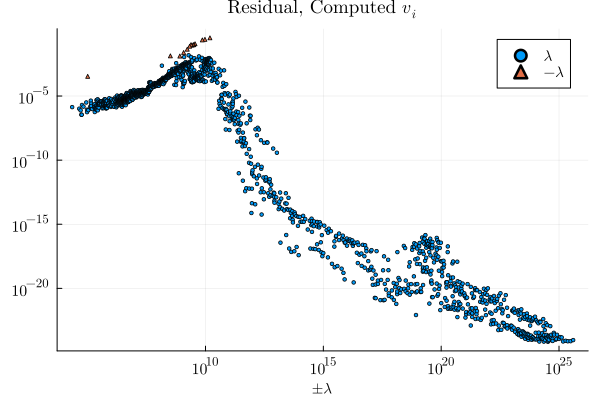
\includegraphics[scale=.25]{./images/pl1_standard.png} 
      & 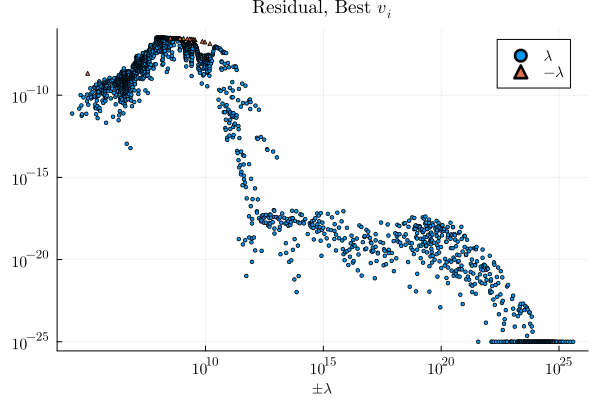
\includegraphics[scale=.25]{./images/pl1_standard_cond.png}
    \end{tabular}
  \end{figure}
\end{frame}


\begin{frame}[allowframebreaks]{Outline}
  \frametitle{Spectral Transformation Lanczos($LU$ Decomposition)}
  
  \begin{figure}
  	\caption{Residuals plot with moderate shift $\sigma=1.5 \times 10^3$}
  	\vspace{1ex}
  	\begin{minipage}{0.45\textwidth} % Adjust the width to control spacing
  		\centering
  		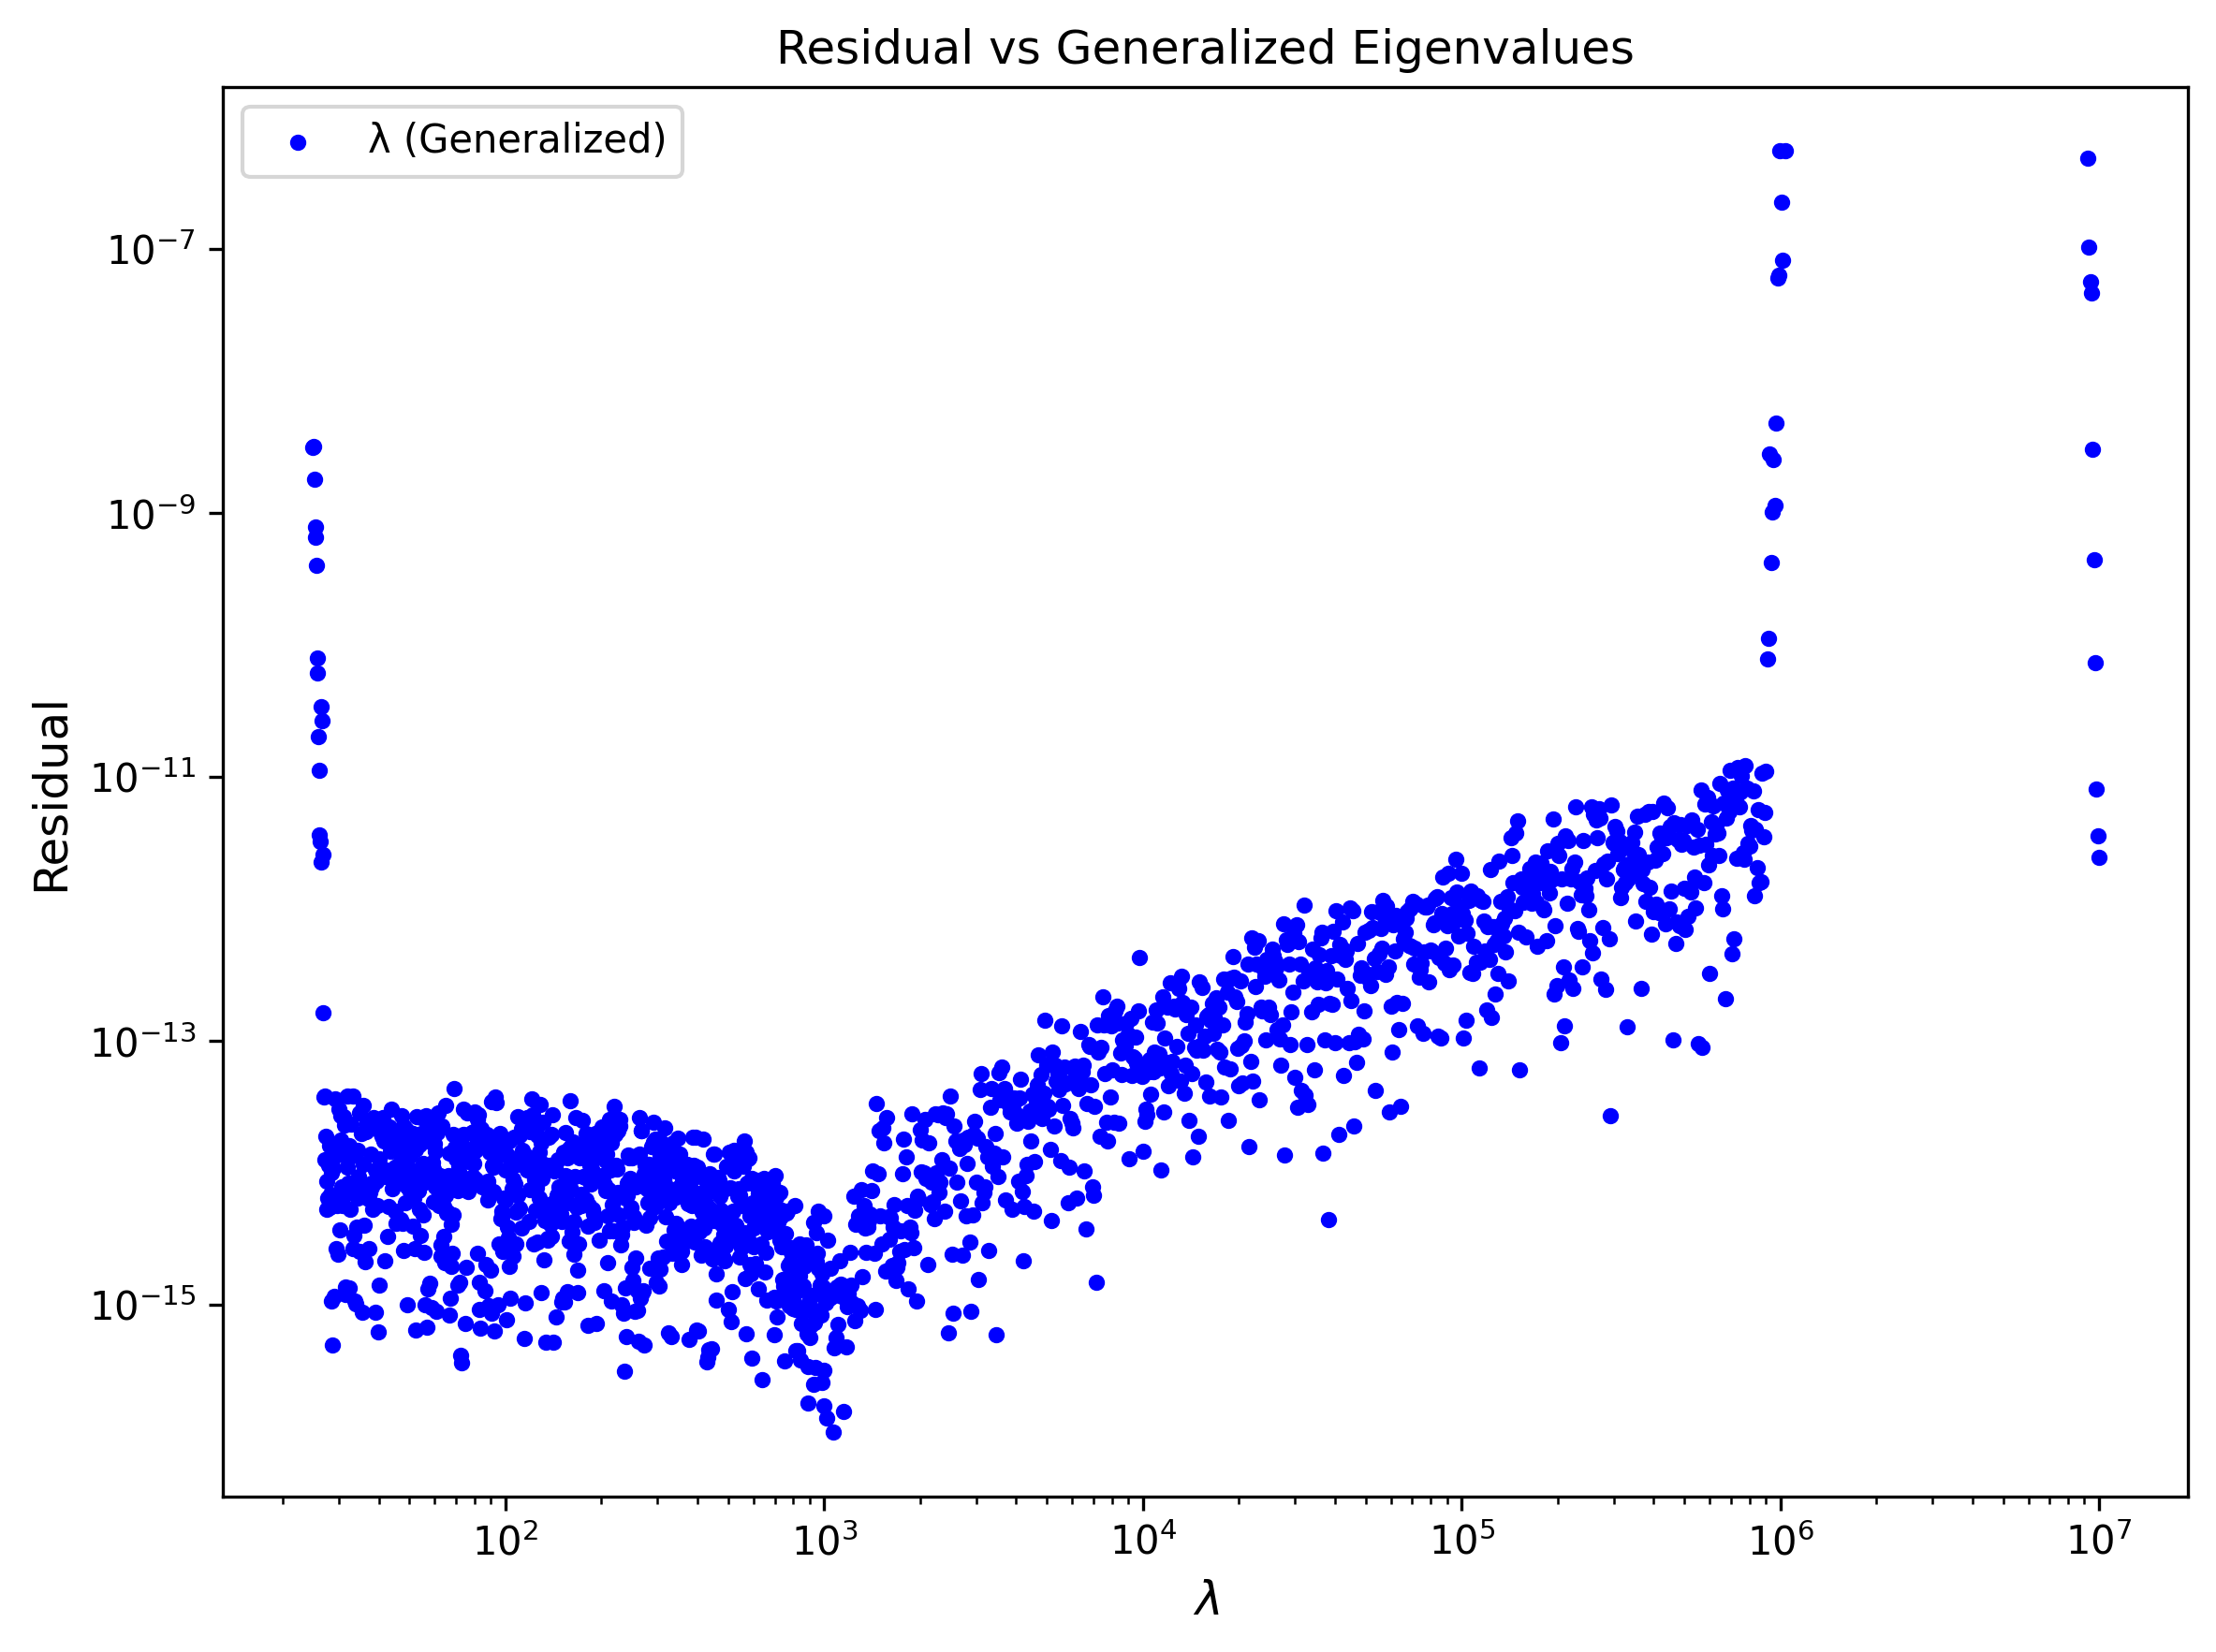
\includegraphics[scale=.25]{./Plots/LU/residual_lu_gs.png}
  		\subcaption{}
  	\end{minipage}%
  	\hfill
  	\begin{minipage}{0.45\textwidth}
  		\centering
  		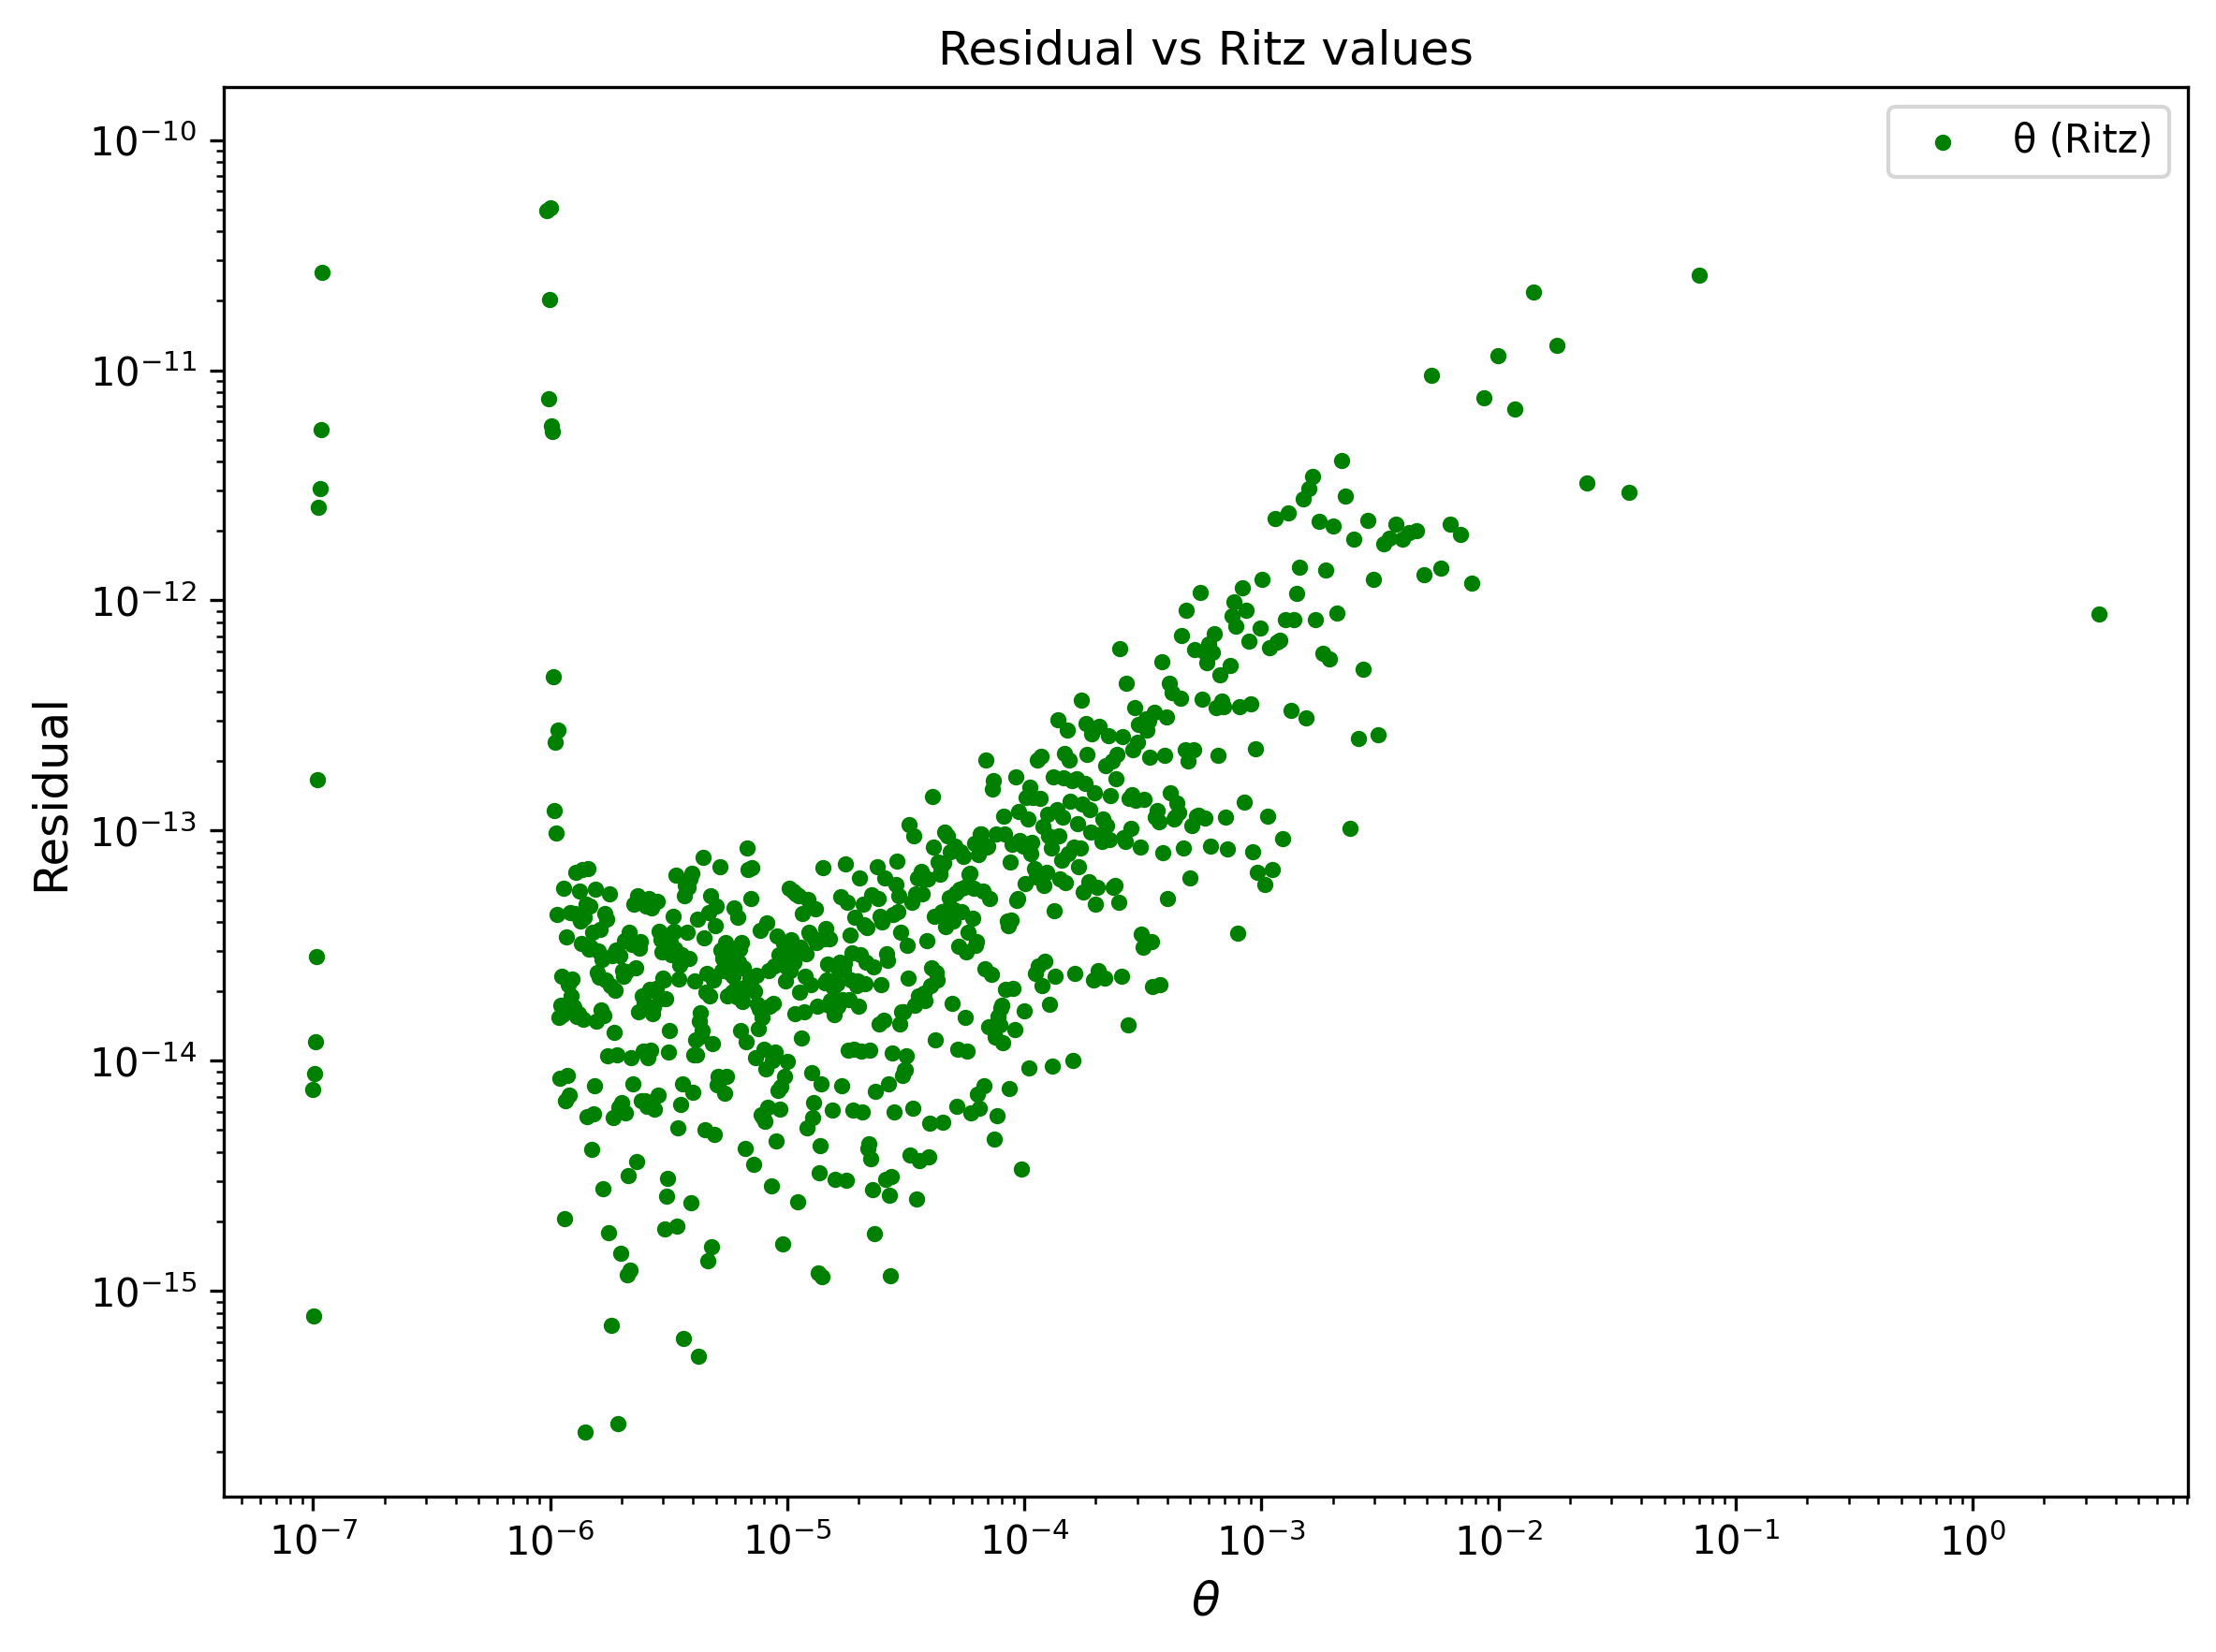
\includegraphics[scale=.25]{./Plots/LU/residual_lu_rs.png}
  		\subcaption{}
  	\end{minipage}
  	
  	\vspace{2ex}  % Adjust the space between rows of images
  	
  	\centering
  	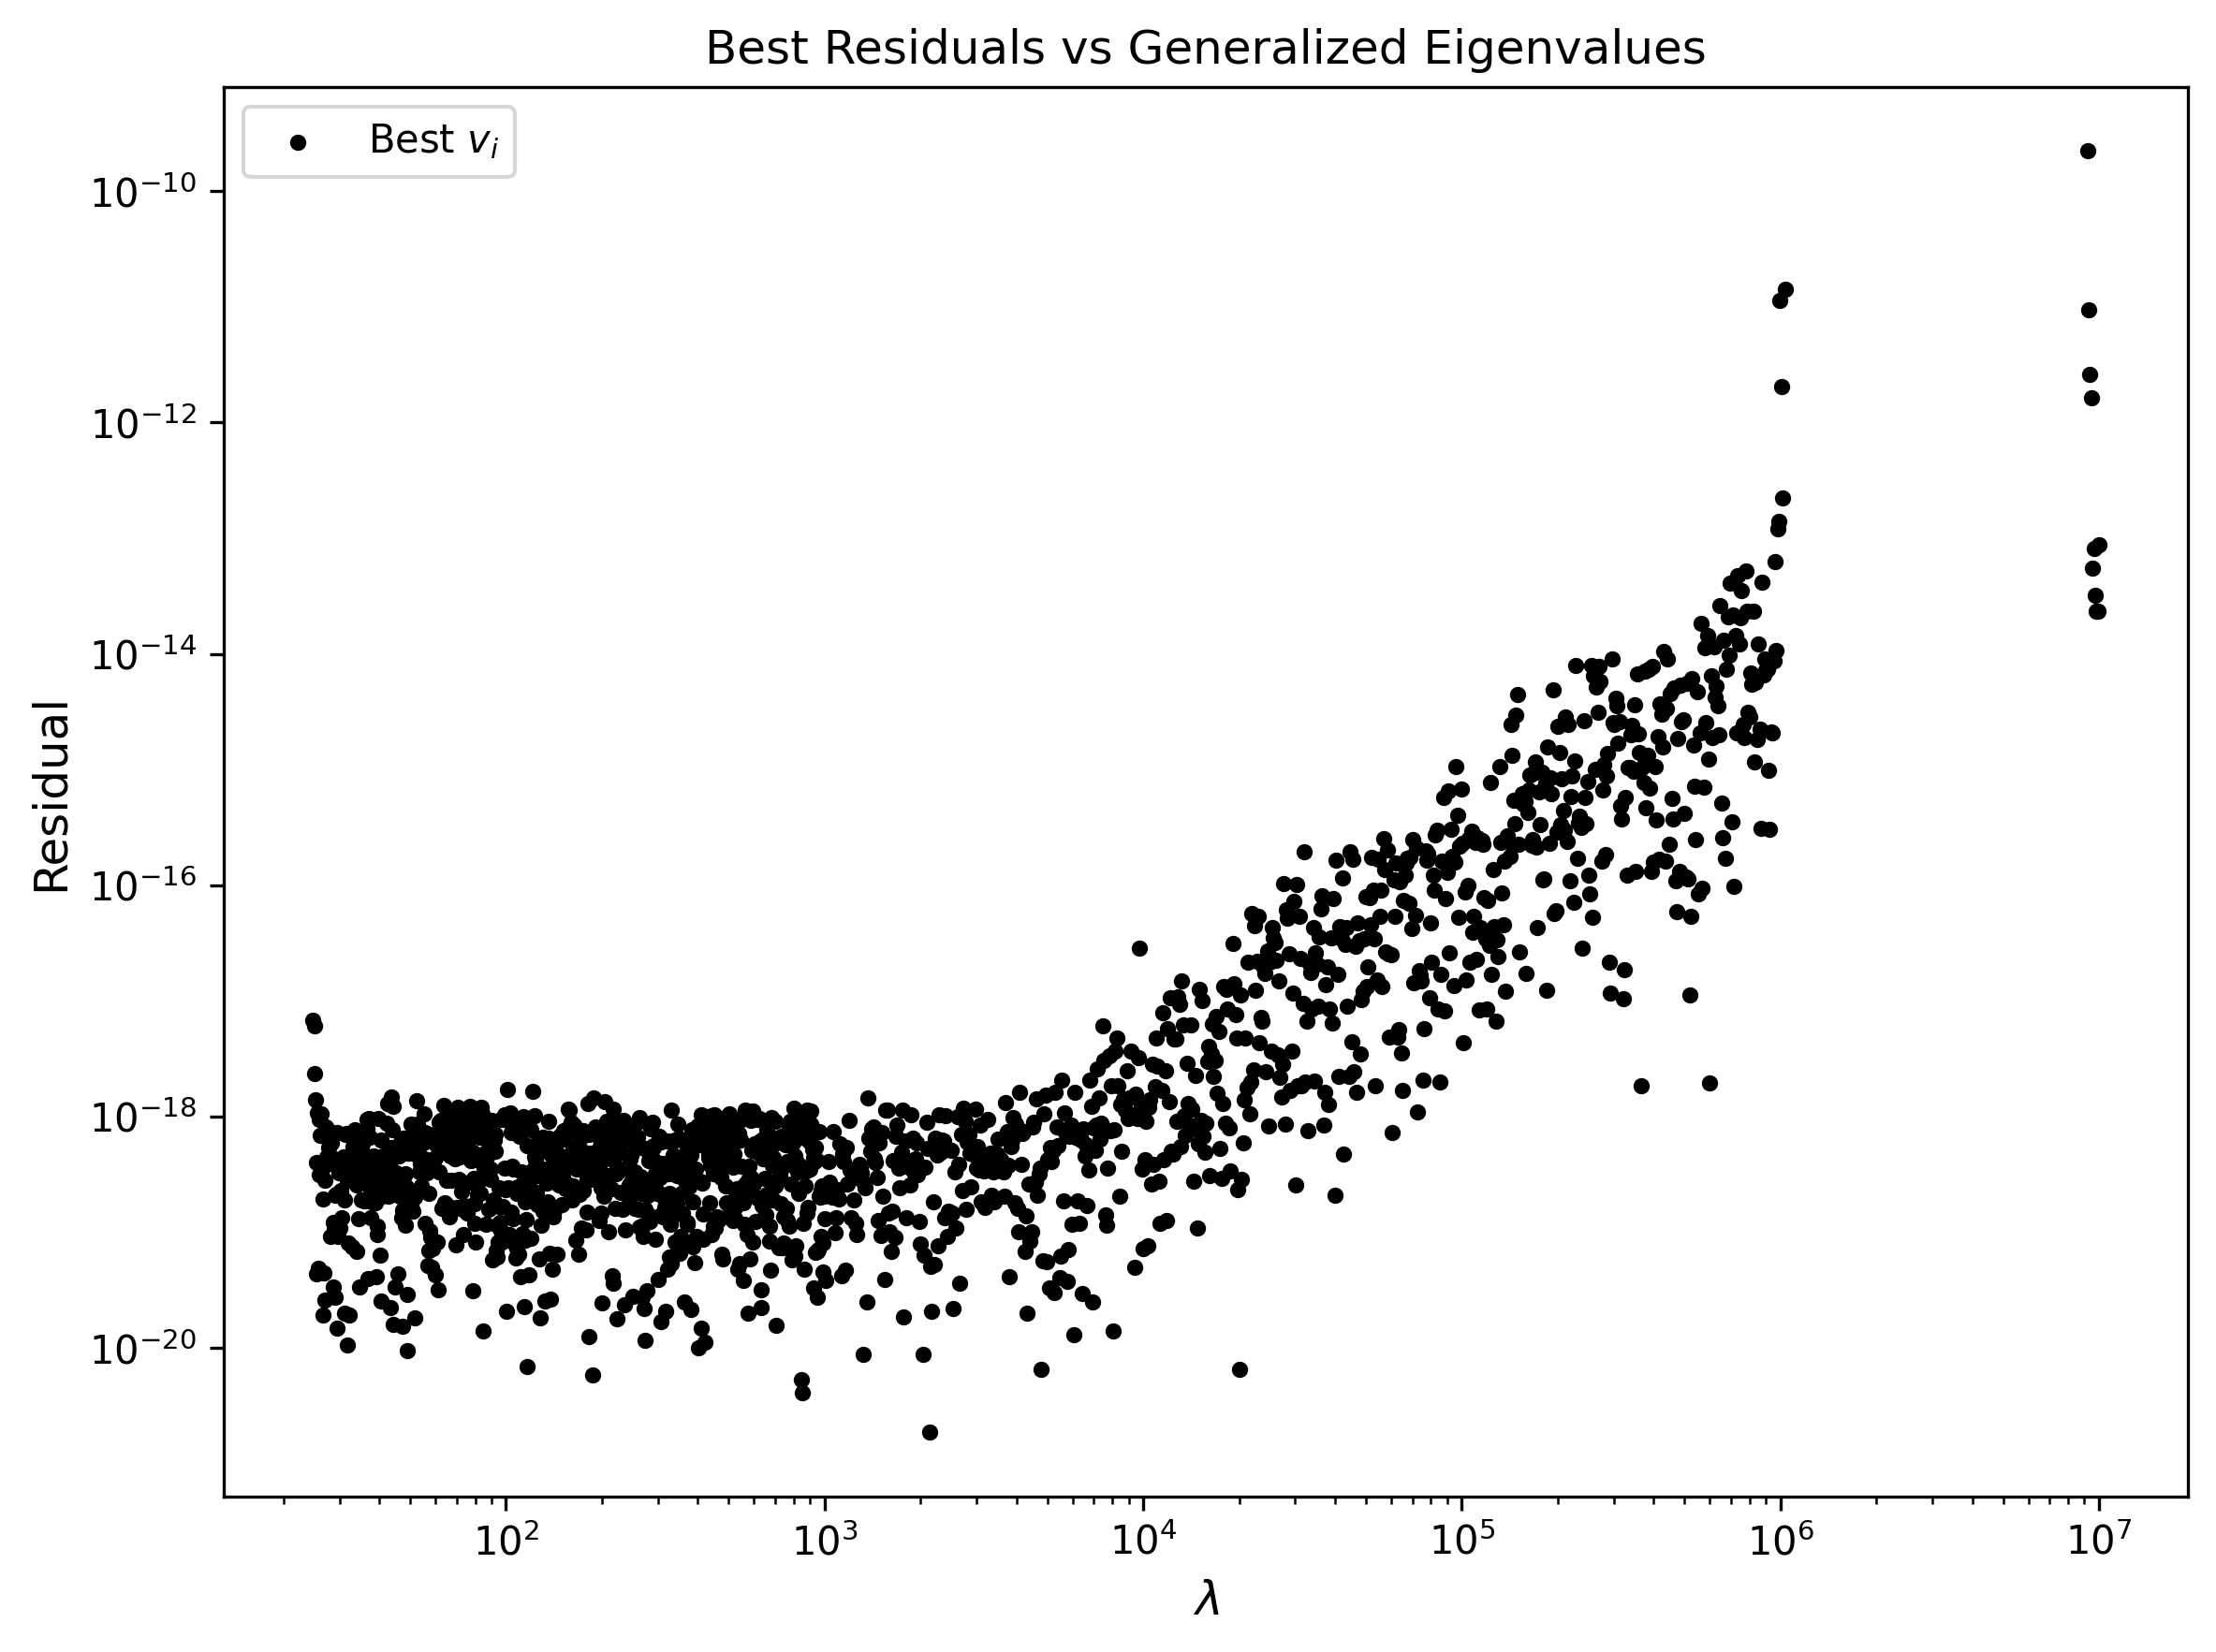
\includegraphics[scale=.25]{./Plots/LU/residual_lu_bs.png}
  	\subcaption{}
  \end{figure}
 
  
  The computation gave the decomposition residual as $6.63 \times 10^{-11}$. Plot ($a$) is the generalized relative residual with the curve given by
  $10^{-14}|1-\lambda_i/\sigma|$. Plot ($b$) is the relative Ritz residuals. Plot ($c$) is the best achievable residual for an idealized eigenvector.
\end{frame}

\begin{frame}[allowframebreaks]{Outline}
  \frametitle{Spectral Transformation Lanczos($LU$ Decomposition)}

\begin{figure}
	\caption{Residuals plot with large shift $\sigma=1.5 \times 10^5$}
	\vspace{1ex}
	\begin{minipage}{0.45\textwidth} % Adjust the width to control spacing
		\centering
		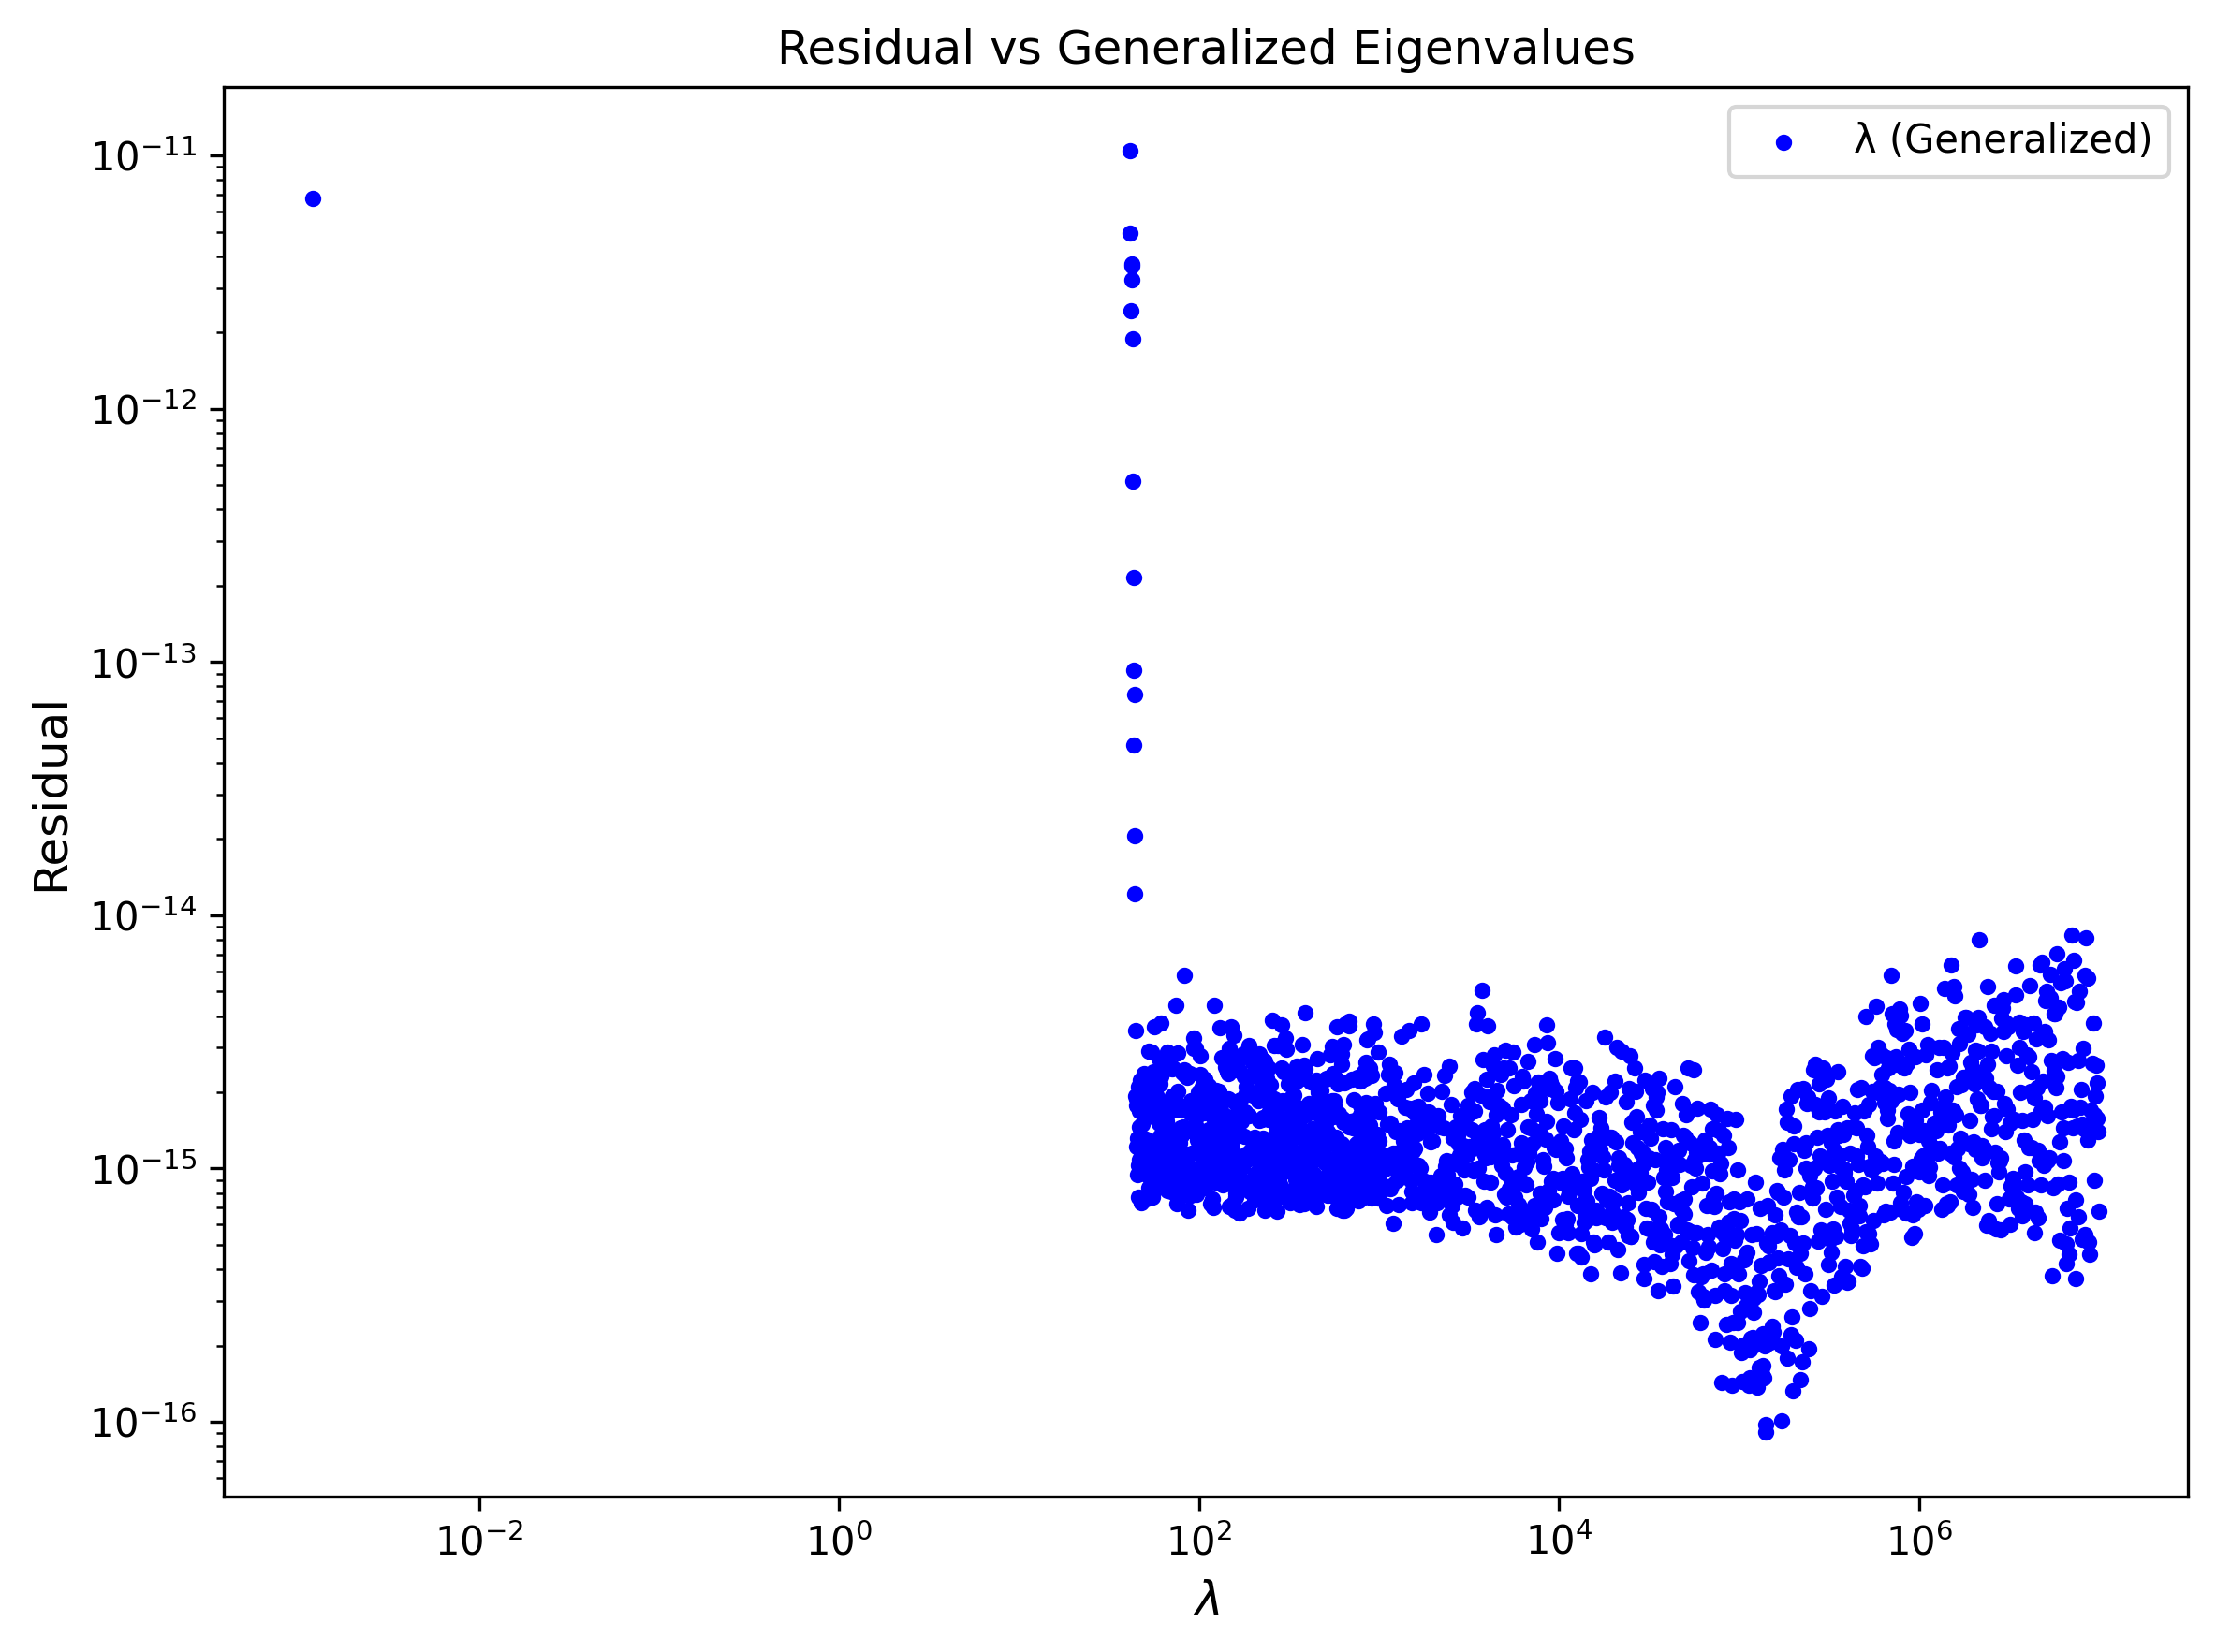
\includegraphics[scale=.25]{./Plots/LU/residual_lu_gl.png}
		\subcaption{}
	\end{minipage}%
	\hfill
	\begin{minipage}{0.45\textwidth}
		\centering
		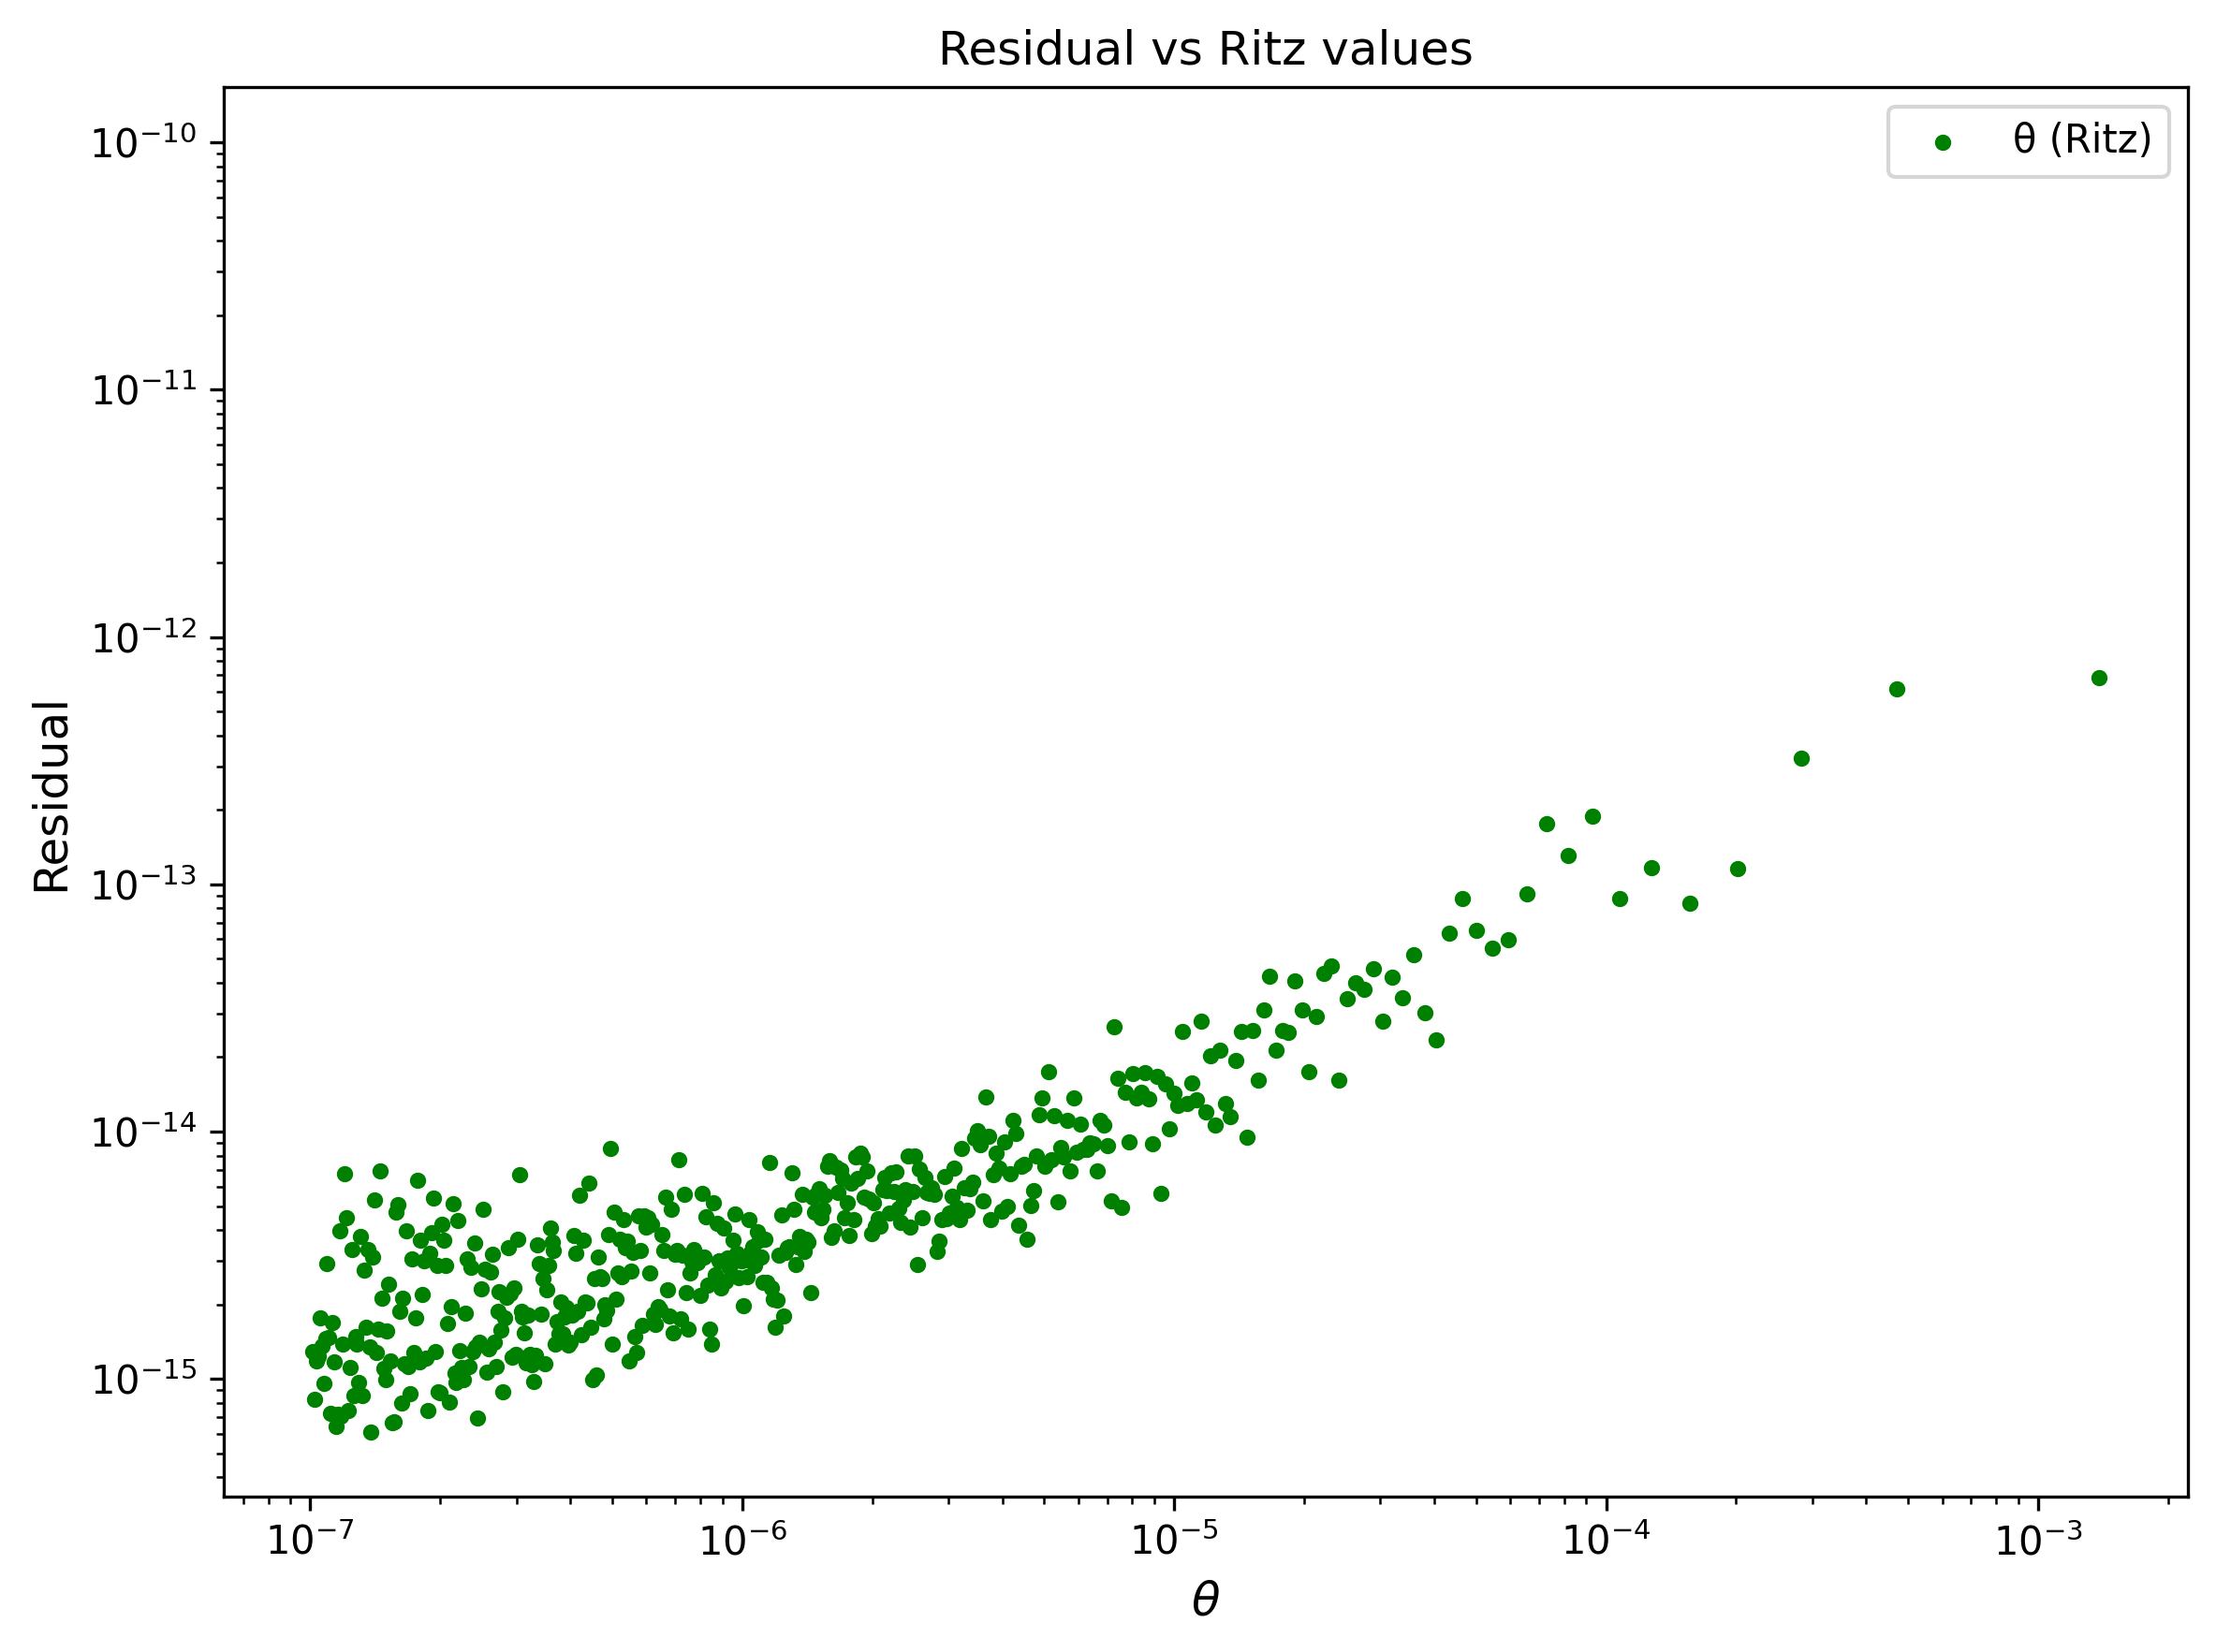
\includegraphics[scale=.25]{./Plots/LU/residual_lu_rl.png}
		\subcaption{}
	\end{minipage}
	
	\vspace{2ex}  % Adjust the space between rows of images
	
	\centering
	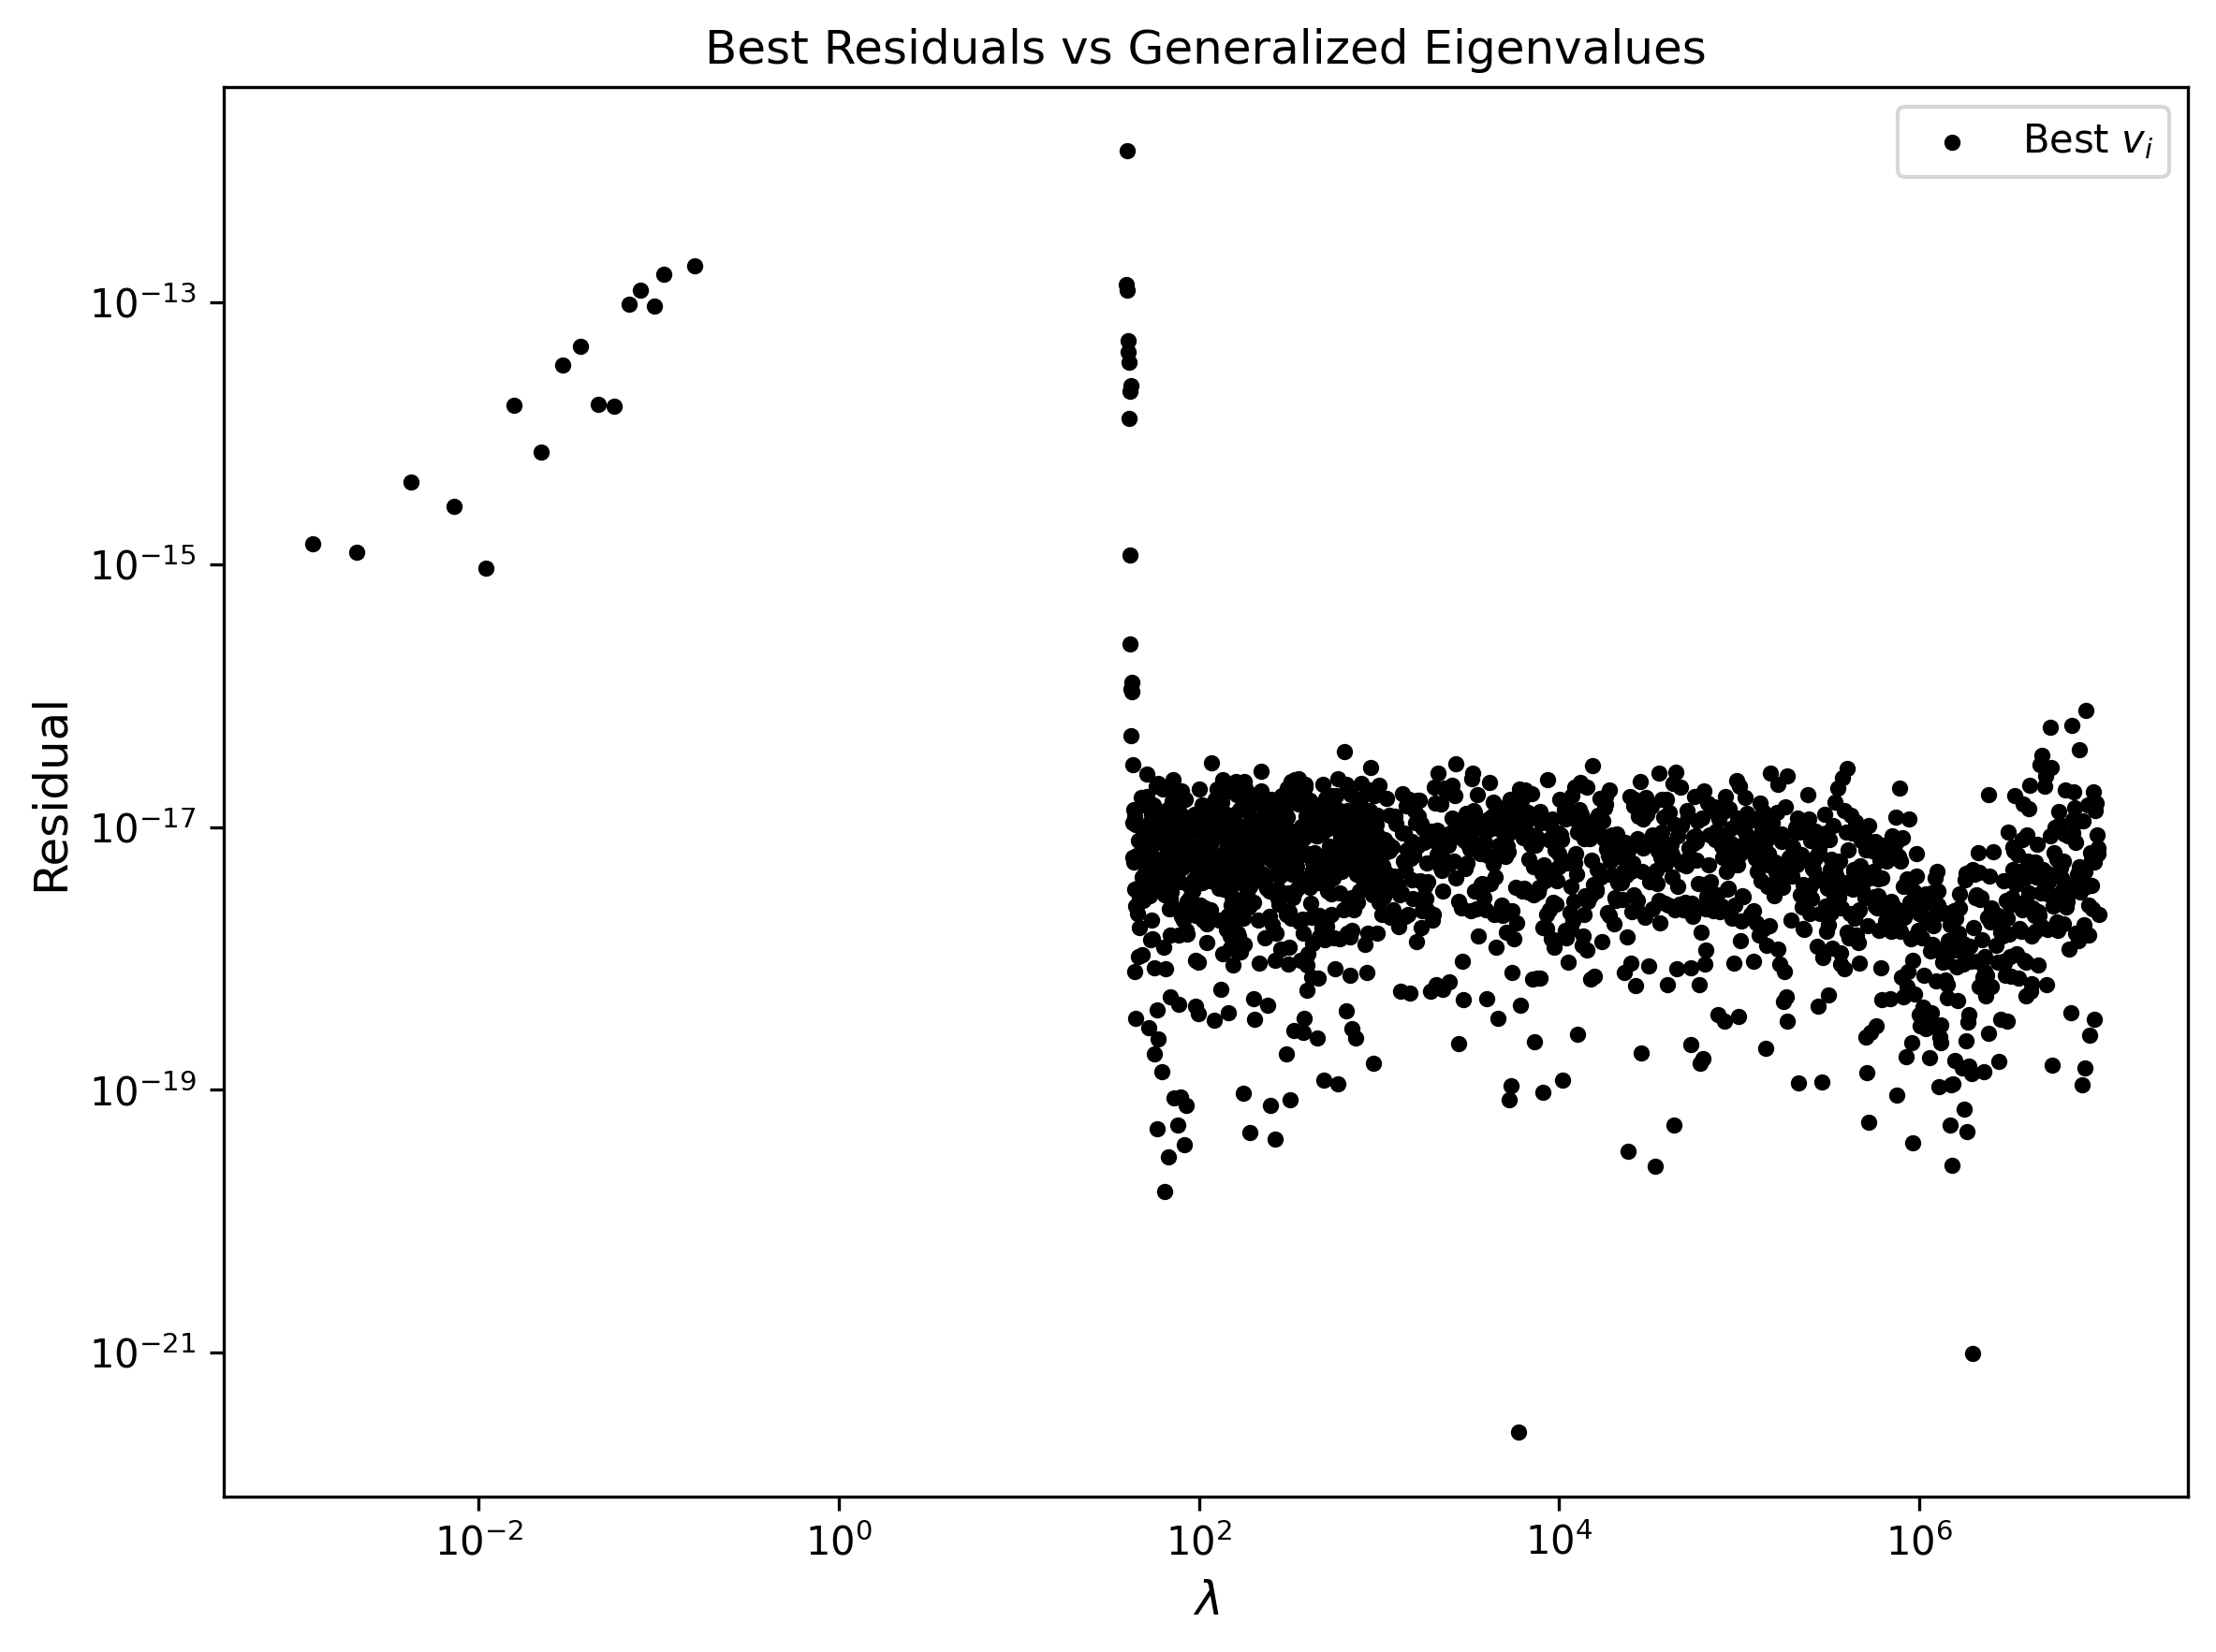
\includegraphics[scale=.25]{./Plots/LU/residual_lu_bl.png}
	\subcaption{}
\end{figure}

  The computation gave the decomposition residual as $5.42 \times 10^{-12}$. Plot ($a$) is the generalized relative residual with the curve given by
 $10^{-15}|(1-\lambda_i/\sigma)(1-\sigma/\lambda_i)|$. Plot ($b$) is the relative Ritz residuals. Plot ($c$) is the best achievable residual for an idealized eigenvector.
\end{frame}


\begin{frame}[allowframebreaks]{Outline}
	\frametitle{ST Lanczos with Eigenvalue Decomposition}
	
\begin{figure}
	\caption{Residuals plot with small shift $\sigma=1.5 \times 10^3$}
	\vspace{1ex}
	\begin{minipage}{0.45\textwidth} % Adjust the width to control spacing
		\centering
		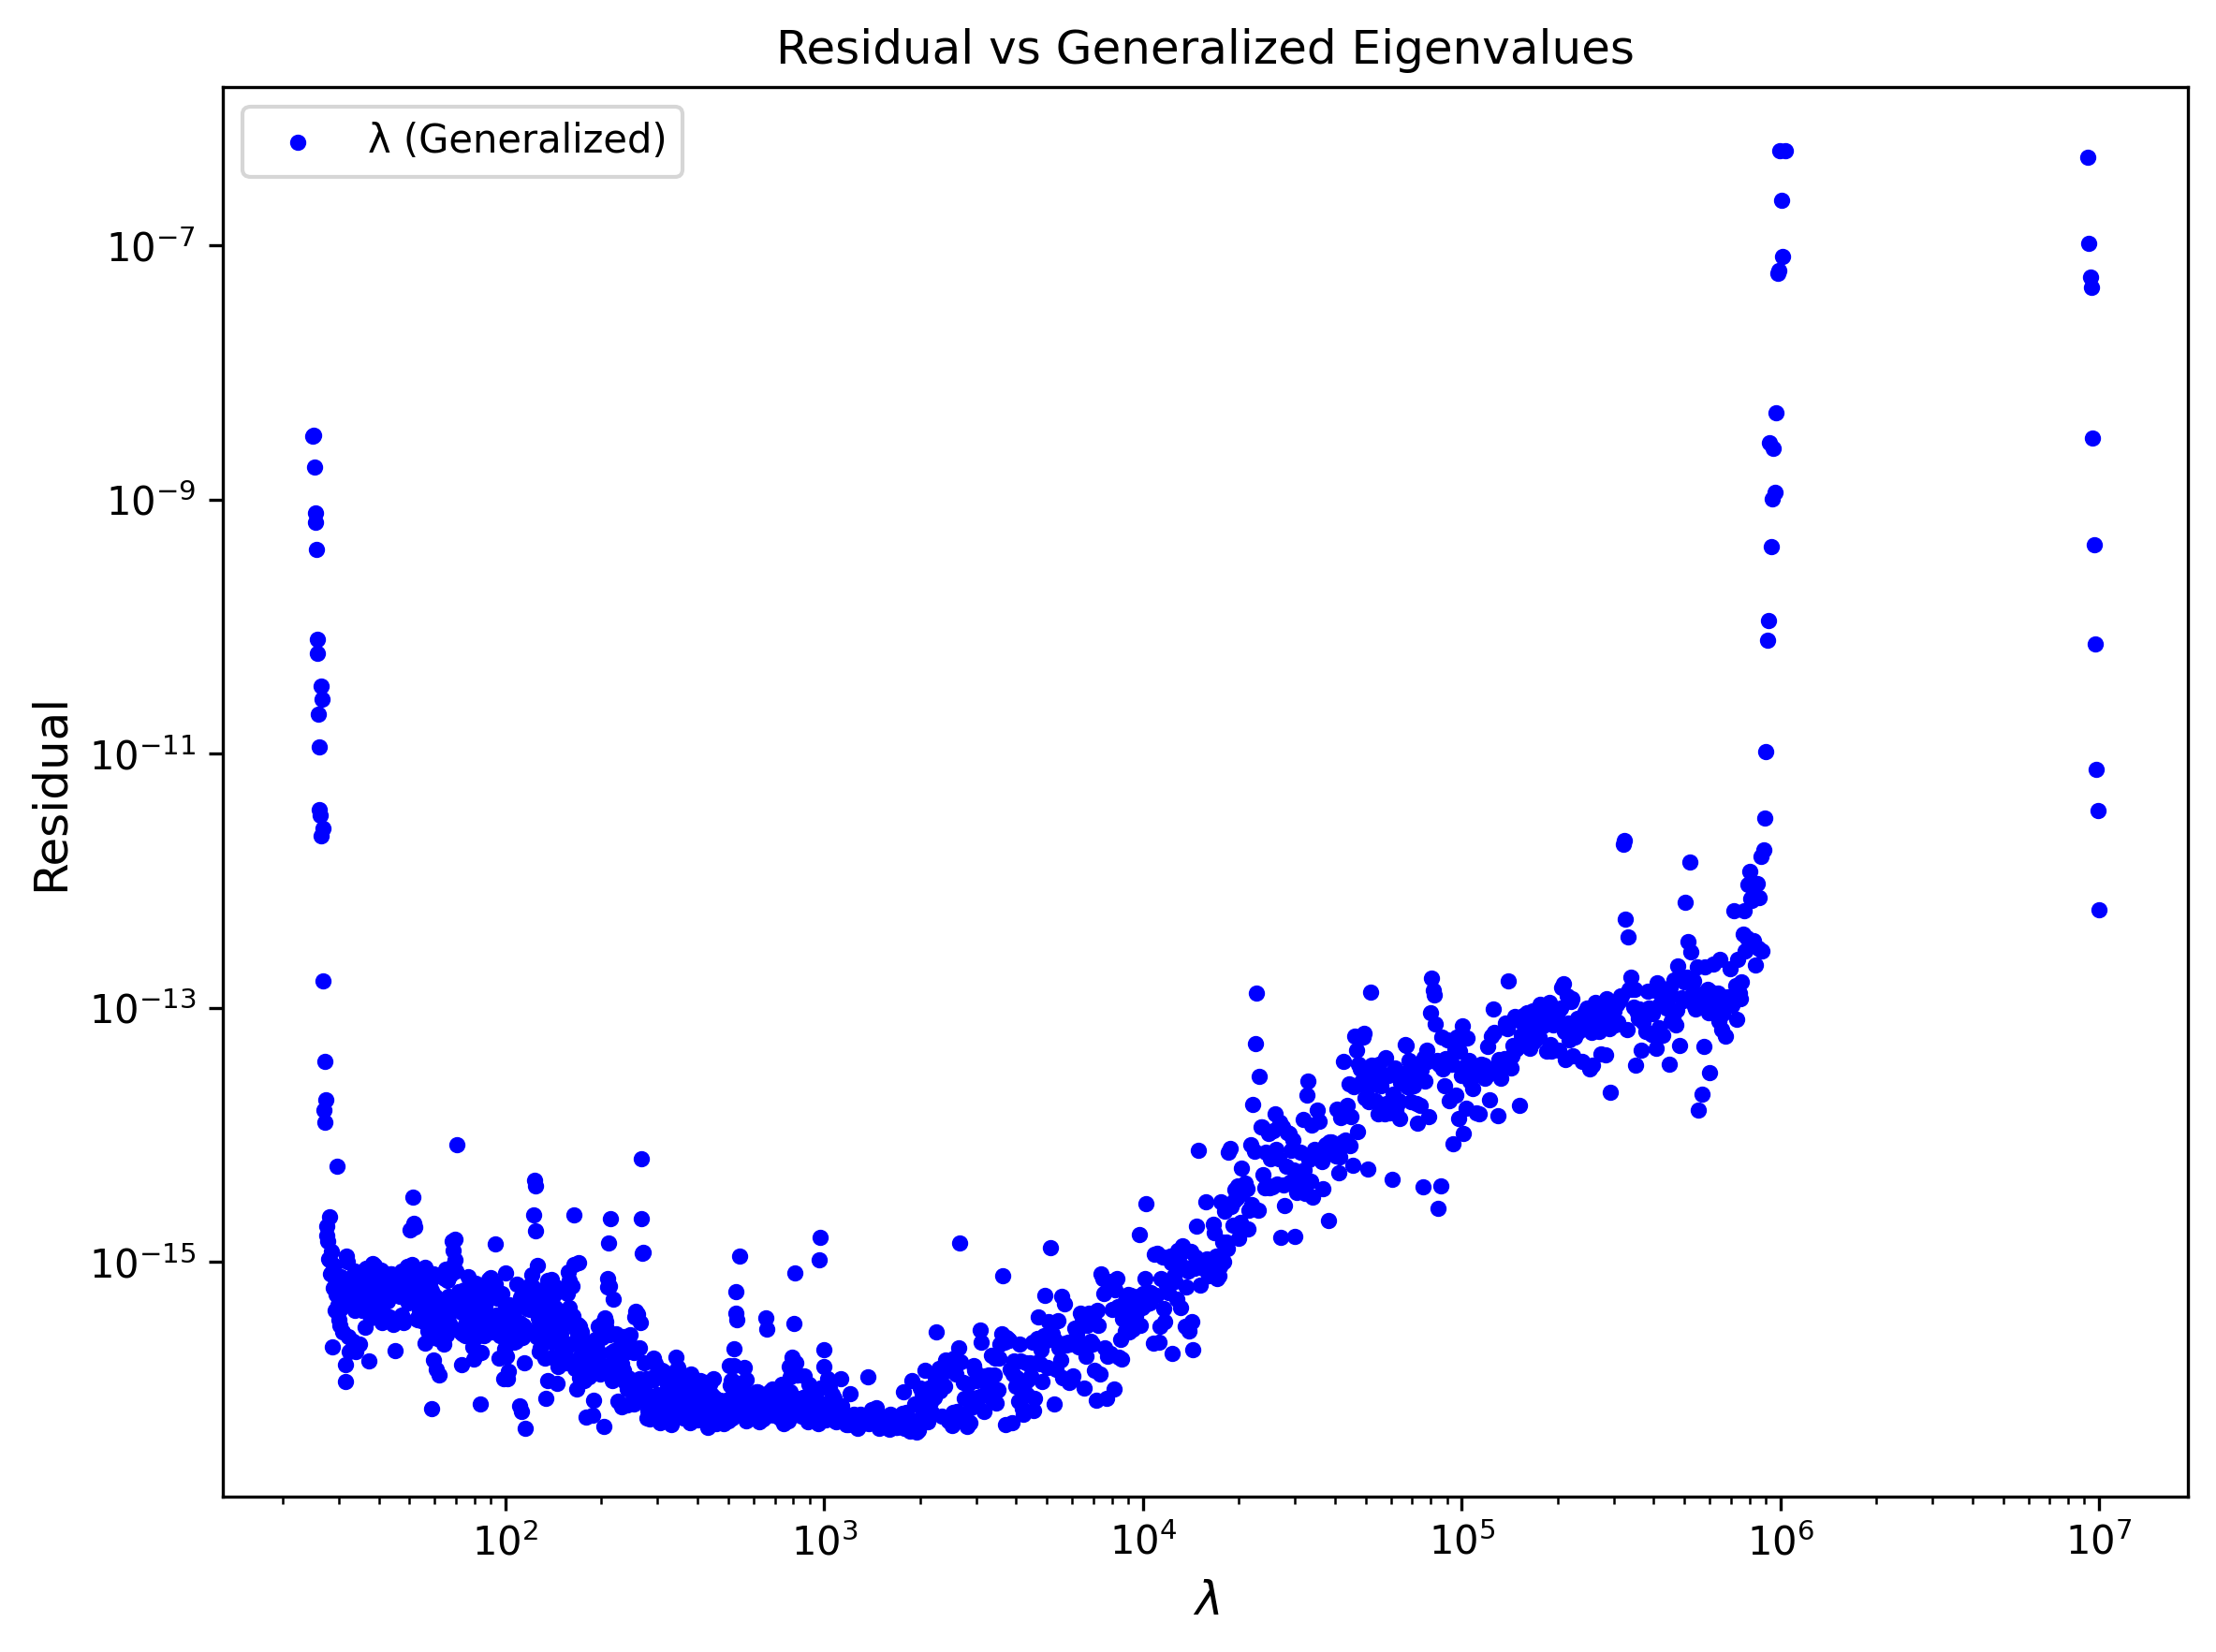
\includegraphics[scale=.25]{./Plots/eigdecomp/residual_eig_gs.png}
		\subcaption{}
	\end{minipage}%
	\hfill
	\begin{minipage}{0.45\textwidth}
		\centering
		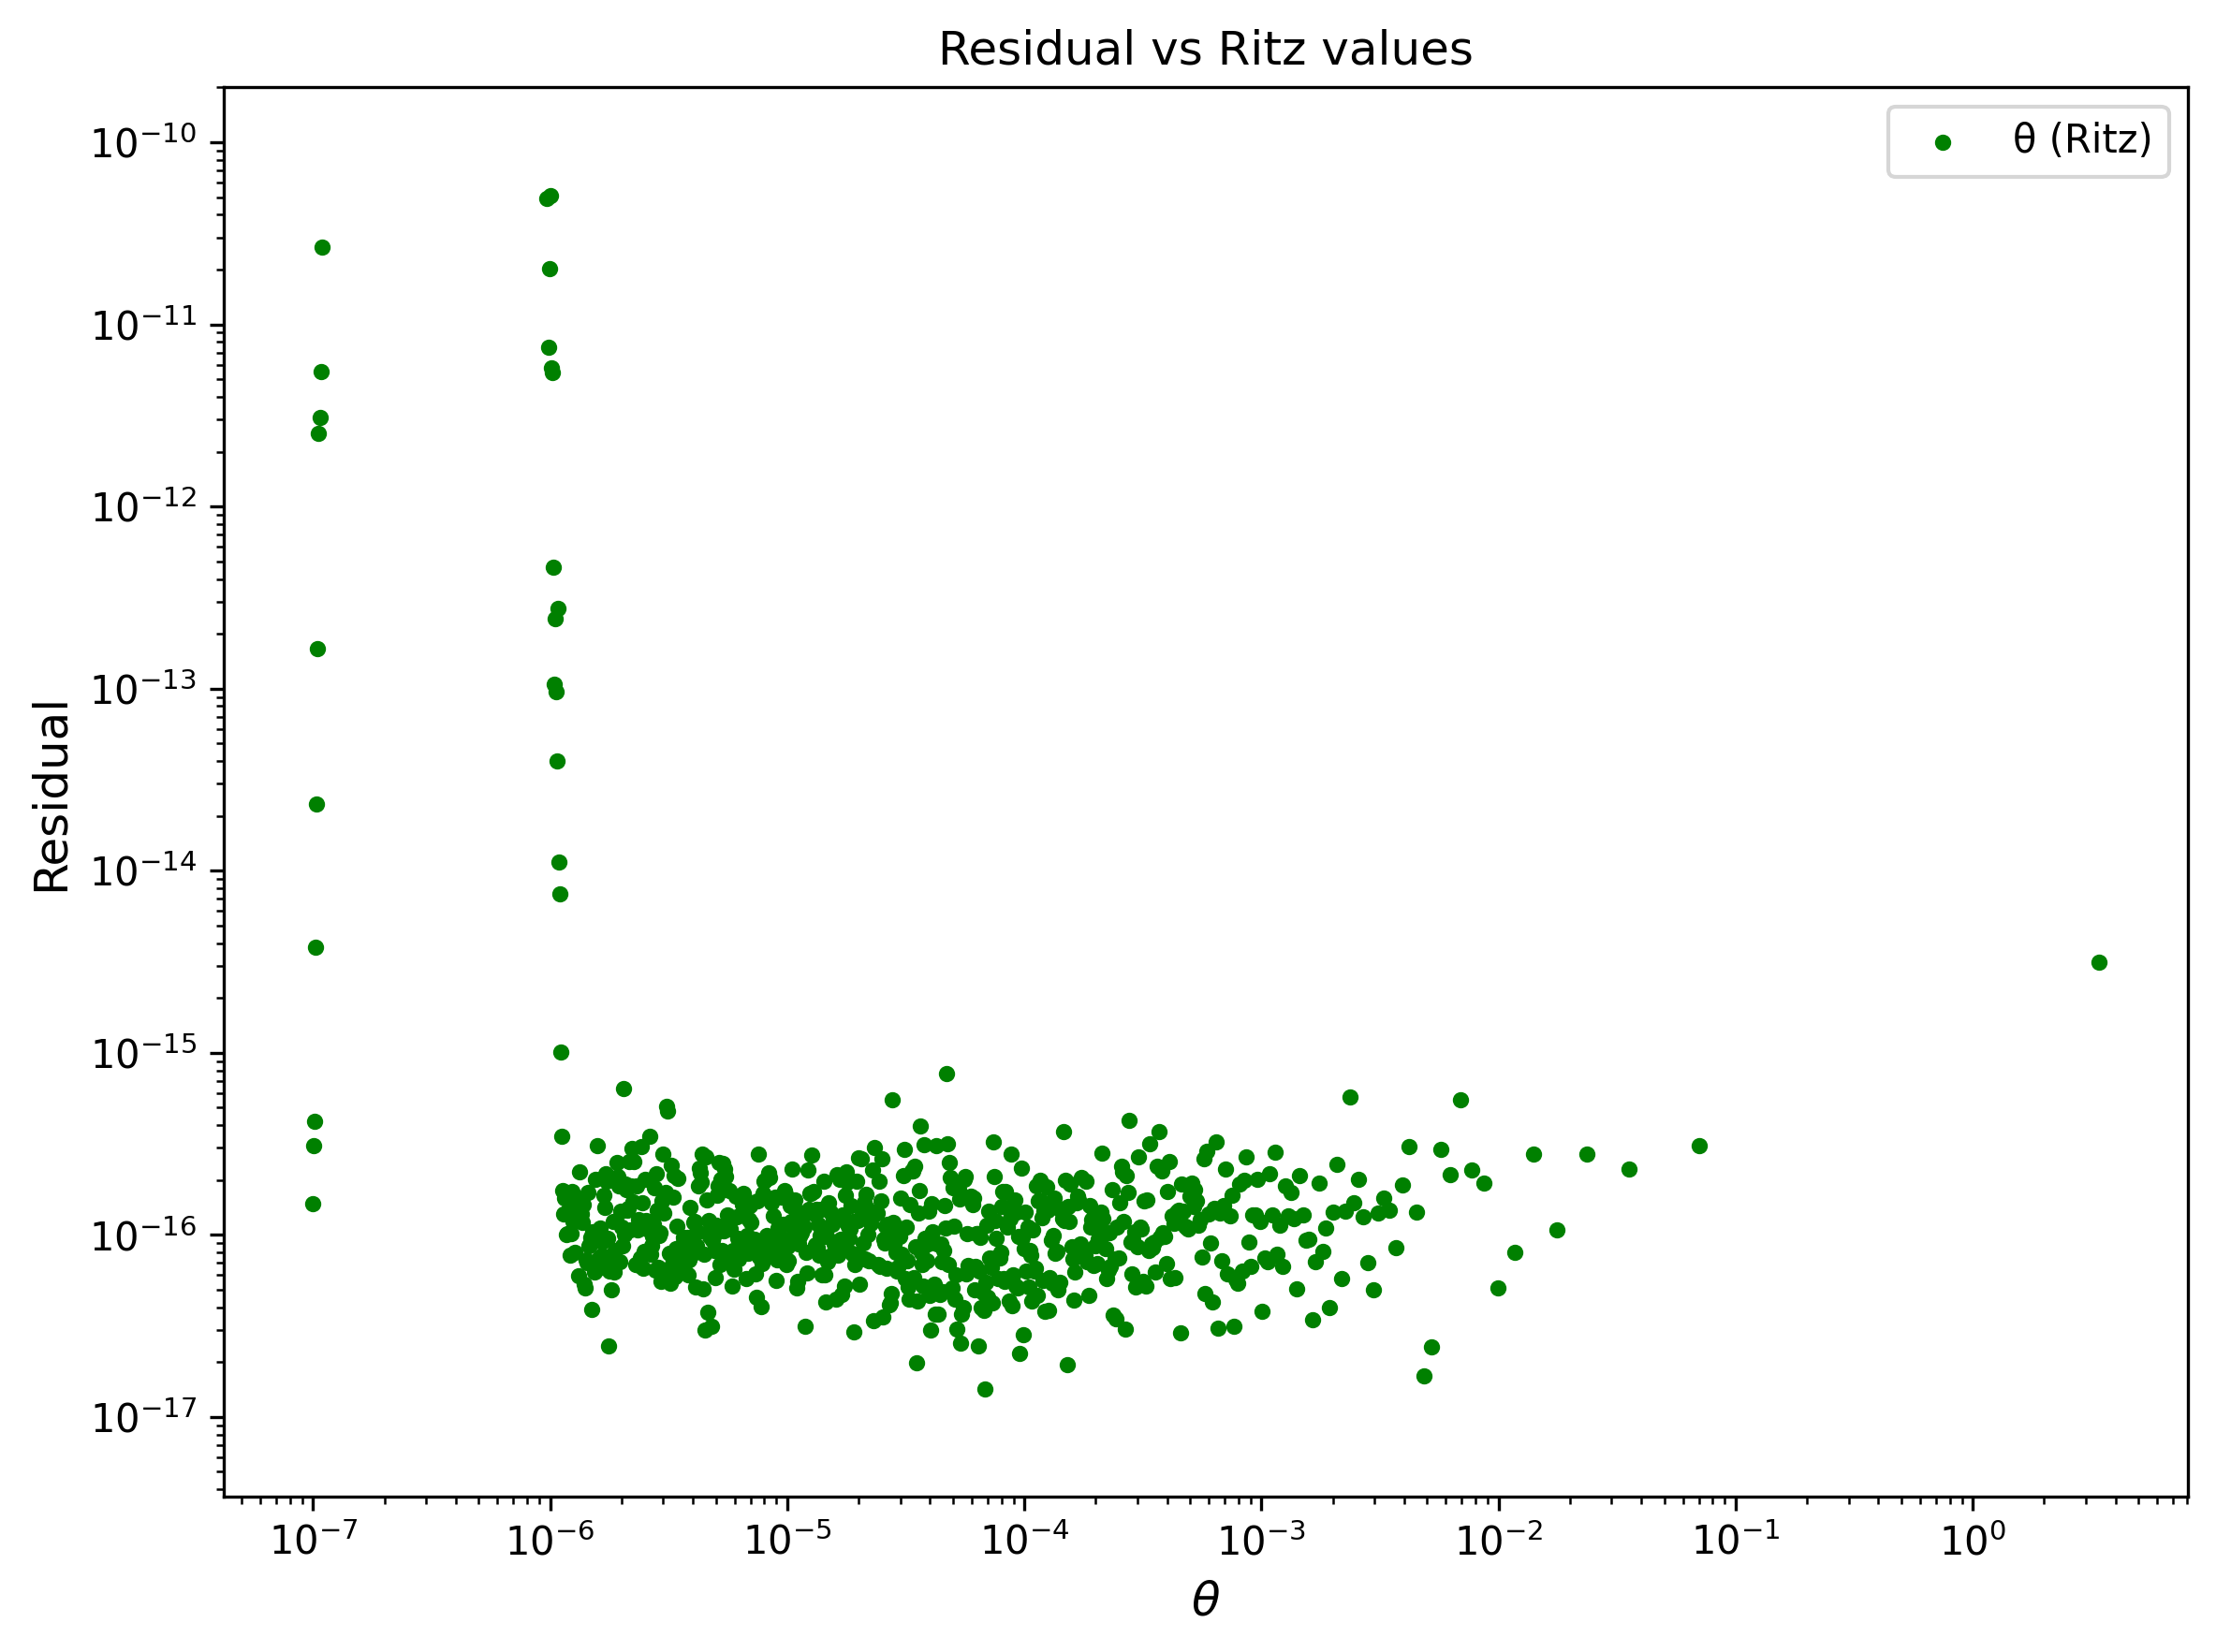
\includegraphics[scale=.25]{./Plots/eigdecomp/residual_eig_rs.png}
		\subcaption{}
	\end{minipage}
	
	\vspace{2ex}  % Adjust the space between rows of images
	
	\centering
	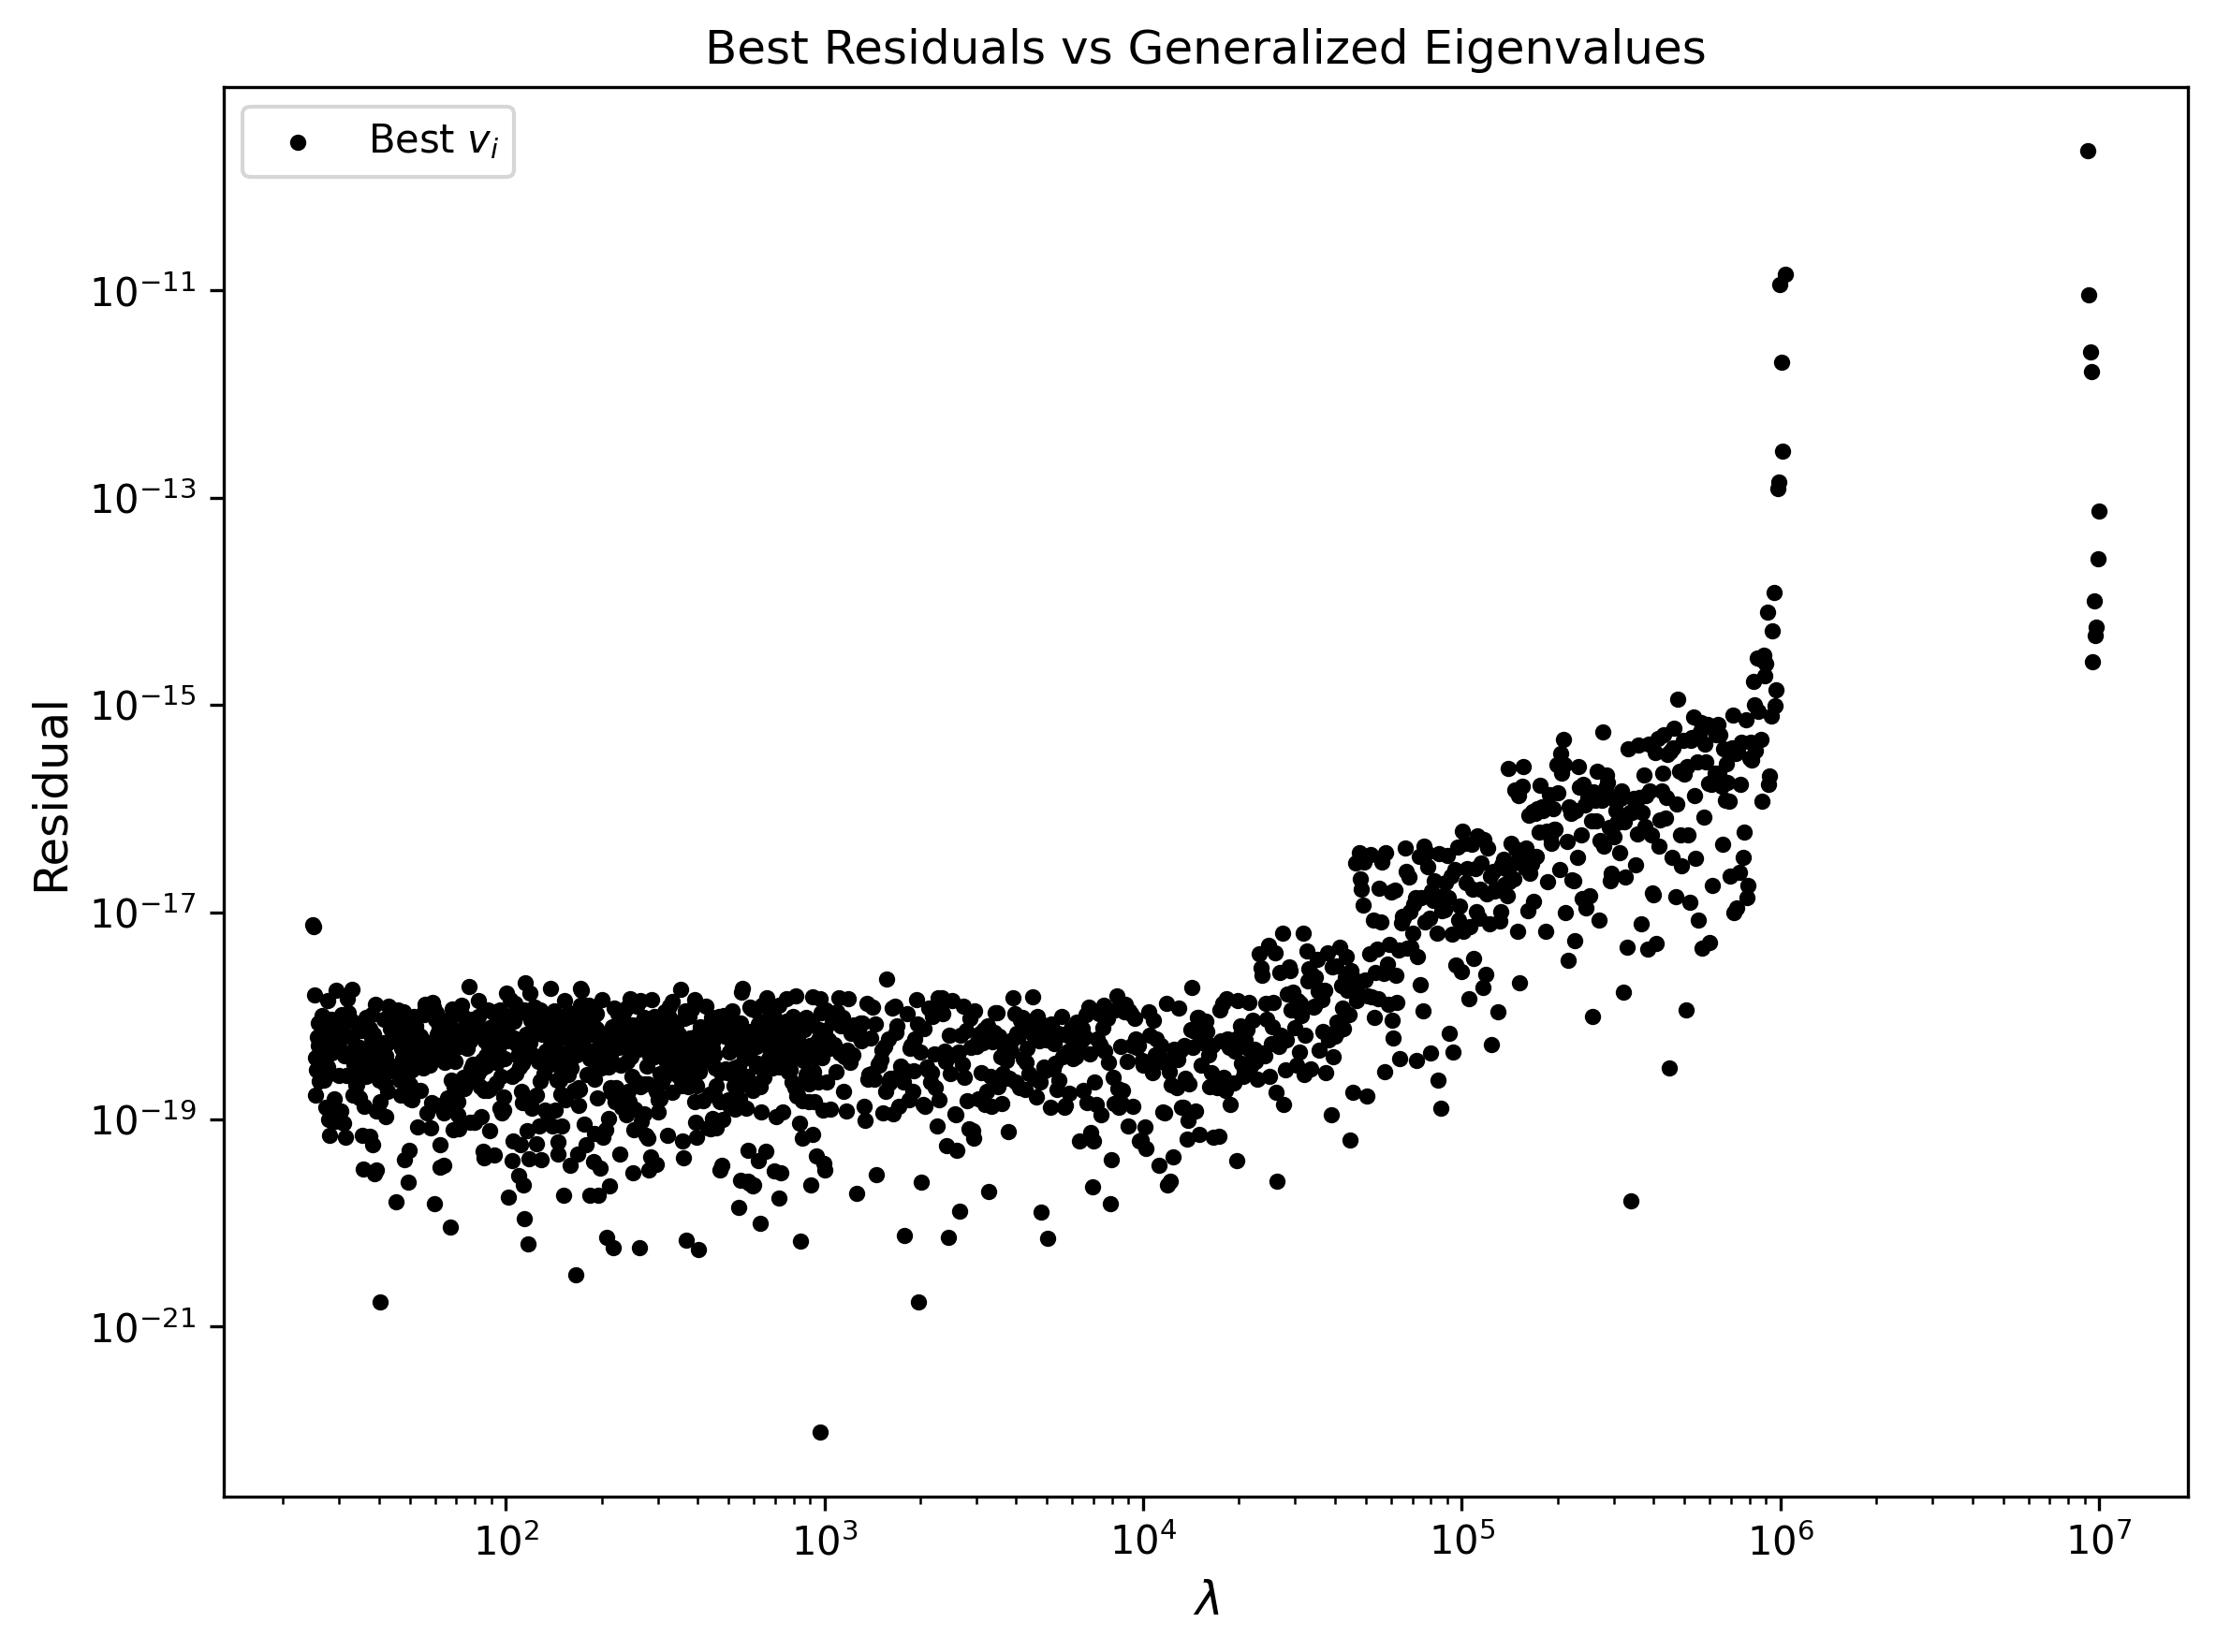
\includegraphics[scale=.25]{./Plots/eigdecomp/residual_eig_bs.png}
	\subcaption{}
\end{figure}
	
	The computation gave the decomposition residual to the order of $10^{-29}$. Plot ($a$) is the generalized relative residual which shows lower residual to the order of unit round off $u \approx10^{-16}$ for eigenvalues close the shift as compared to an $LU$ decomposition. Plot ($b$) is the relative Ritz residuals. Plot ($c$) is the best achievable residual for an idealized eigenvector.
\end{frame}
\begin{frame}
  \frametitle{Pros and Cons}
  
  {\bf Pros:}
  \begin{itemize}
  \item The algorithm is fast for sparse matrices since it uses Lanczos algorithm which is $O(nm^2 + n^2m)$.
  \item It is efficient in computing a subset of eigenvalues, making it memory efficient.
  \item Since all the work is done in matrix decompositions that are
    implemented in LAPACK, the algorithm is almost as fast as the
    standard method and is easy to implement efficiently, even in a
    slow language.
  \item With a little effort, it can be designed to handles the case of semidefinite $B$ effectively.
  \item Delivers really small residuals for symmetric decompositions.
  \end{itemize}

  {\bf Cons:}
  \begin{itemize}
  \item The eigenvector computation is not unconditionally stable.
  \item Choosing the shift annoying, even if it is relatively easy to
    choose, especially if one wants a black box algorithm.
  \end{itemize}
\end{frame}

\end{document}
